\section{Introduction}

\subsection{Chapter Outline}

In this chapter I use a deterministic compartmental gonotrophic cycle model of vector dynamics to investigate the impact of different vector control methods on key measures of disease transmission, focusing specifically on lymphatic filariasis and malaria. I compare the impact of different vector control methods, including indoor residual spraying (IRS) and larvicides, and then go on to demonstrate how low prevalence could potentially be achieved using long-lasting insecticide nets (LLINs) alone. I show that the dual effect of killing and transmission prevention caused by IRS or LLINs scales up with coverage much faster than the population reduction method of larvicides. I draw parallels between LF and malaria transmission and discuss the potential for collaboration in co-endemic areas.

\subsection{Disclaimer}

The work in this chapter builds on a simple vector model I developed during an MSc research project specifically for modelling the effect of bednets on LF transmission. The model described here and the results presented represent work done during my PhD.

\subsection{Background}

%references from Ross, Macdonald and... Smith 2012
Ronald Ross and George Macdonald are known for their contributions to developing a mathematical model for mosquito-borne disease transmission, with the resulting models often referred to as `Ross-Macdonald' models, and Ross is widely credited for first discovering the transmission of malaria by mosquitoes. In 1904, Ross published a mathematical population model of adult mosquitoes, specifically investigating spatial larval control methods and their impacts on mosquito populations and disease transmission \cite{Ross1905}. Ross argued that multiple methods of control would be necessary in most settings, including larval control, bednets (which were not insecticide treated at the time) and improved housing. The discovery of the insecticidal effects of dichlorodiphenyltrichloroethane (DDT) would later introduce the possibility of IRS, or treating bednets, to reduce mosquito densities in the place of larval control. 

In the 1950s George Macdonald extended and used Ross' malaria models to develop metrics for measuring vector-borne disease transmission. Macdonald's malaria model \cite{Macdonald1957} is still widely cited and used as a basis for further modelling. This theory provided important insights into the relative benefits of certain interventions and laid the groundwork for adult-target vector control to be recognised as the best method for managing malaria \cite{Dye1992,Morrison2008}. Long-lasting insecticide-treated nets (LLINs) have been a widely used method in combating malaria transmission since 2004. They are draped over beds, as peak vector biting activity of a number of mosquito species occurs between dusk and dawn \cite{korgaonkar2012}, and serve to both kill and repel adult vectors. As it is predicted that transmission intensity and geographic viability of vector-borne diseases will increase with climate change, methods for controlling these diseases and their vectors are increasingly important \cite{Watson2005}.

For LF, as seen in Chapter \ref{chap:ELIM}, large-scale preventative chemotherapy has been shown to be effective at achieving elimination as a public health problem in certain settings \cite{de2013,cheun2009}. The majority of national elimination programs focus solely on this approach, as recommended by the World Health Organization guidelines, with mosquito control only considered a supplemental strategy \cite{WHO2019_FactSheet}. However, a key problem is that, of the remaining endemic countries, many at-risk communities are hard to reach and have poor or no access to health care \cite{koudou2014}. We have also seen there is evidence to suggest that, in some settings, these methods alone are insufficient to ensure transmission is interrupted. In Sri Lanka, following an mass drug administration (MDA) program that ran from 2002 to 2006, a observational study has shown persistence of low-level LF transmission \cite{rao2014}.

Whilst vector control has been cited as a possible supplementary preventative tool to be used in parallel with MDA \cite{WHO2019_FactSheet}, its importance may still be underestimated; correct usage of vector control could reduce the number of rounds required to interrupt transmission, whilst also aiding the prevention of disease resurgence \cite{bockarie2009}. Additionally, in The Gambia, there is evidence that transmission was interrupted in the absence of MDA due to malaria-focused vector control programs, specifically following the use of LLINs \cite{rebollo2015}. The Gambia has had a varied history of LF prevalence, with a high of an estimated 50\% of adults being mf positive in the 1950s. Despite no distribution of anti-filarial drugs, surveys in the 1970s showed prevalence had halved in the worst affected areas and prevalences as low as 2.9\% were recorded in some locations \cite{knight1980}. This decrease was attributed to reductions in mosquito biting rates, due to a combination of lower rainfall and the introduction of LLINs. A later study, considering data spanning from 1997 to 2013 \cite{rebollo2015}, found that LF transmission may have been interrupted in The Gambia during this time and attributed this interruption to the rapid scale up of LLIN usage.

With similar anecdotal results in Papua New Guinea \cite{Reimer2013_insecticidal}, in addition to Nigeria launching a plan to coordinate malaria and LF elimination programs in 2014, using LLINs as a key component \cite{Nigeria,richards2013}, there is an increasing awareness of the impact that vector control can have on elimination programs. The results from The Gambia, in particular, demonstrate it may be possible to achieve elimination in some settings using just vector control, as we might expect from the theoretical discussion around breakpoints in the previous chapter (low vector density will result in lower worm burdens, and hence less chance of parasite sexual reproduction, making transmission less sustainable). The cross-disease benefit could also pose an attractive prospect for countries endemic with both malaria and LF. However, this may not be achievable within feasible time frames and the effect will vary with local transmission conditions.

LF and malaria share common vectors, meaning vector-based malaria control methods will also combat LF transmission. The success of LLINs in the global malaria effort has made them arguably the most important current tool for malaria control in Africa \cite{killeen2007}. We would theoretically expect them to be even more effective against LF, as it is less transmissible than malaria. Due to a lower probability of infection given one infectious bite \cite{bogh1998}, sustained LF transmission requires a higher biting rate.

\subsection{Modelling}

Ross' first model of mosquito-borne disease transmission, published in 1908 \cite{Ross1908}, was a description of the expected number of human infections based on the number of mosquitoes and the mosquito infection dynamics. Between each time step (defined as one month), he assumed that a mosquito could take two bloodmeals, enough to contract the infection and then transmit it back to another human. His main conclusions from this were in noticing a relationship between the mosquito to human ratio and the number of human infections, particularly that there was a critical mosquito density below which transmission would not be sustained. His second model was a coupled set of differential equations for the number of infectious humans, $X$, and the number of infectious mosquitoes, $Z$ \cite{Ross1911}.

In 1923, Lotka and Sharpe extended this second model to include the extrinsic incubation period (EIP) in the mosquito and the intrinsic incubation period (IIP) in the human \cite{Lotka1923}. Macdonald's development of the model, however, is the most well-known and was the first to describe the recovery rate under superinfection. Macdonald also derived a formula for the basic reproduction number ($R_0$) for mosquito-borne diseases, the number of secondary cases generated by one infectious case in a totally susceptible population:

\begin{equation}
    R_0 = \frac{m a^2 b c p^v}{-r\log{p}}\,.
\end{equation}

where $m$ is the ratio of mosquitoes to humans, $a$ is the daily blood feeding rate, $b$ is the proportion of infectious bites than infect a human, $c$ is the opposite, the proportion of bites on an infectious host that infect a mosquito, $v$ is the extrinsic incubation period, $r$ is the human recovery rate and $p$ is the daily mosquito survival probability \cite{Macdonald1957}. 

In contrast, as a lesser studied disease, there was little attempt to model LF transmission until the 1990s; this decade saw the formulation and publication of three models \cite{Rochet1990,Chan1998,Plaisier1998}. The first, published in 1990, was a simple deterministic differential equation model \cite{Rochet1990} of prevalence in the vector population and mean worm burden in the human population. This was followed by two more in 1998: EPIFIL, a determinisitic population-level model \cite{Chan1998}, and LYMFASIM, a stochastic individual-based model \cite{Plaisier1998}. EPIFIL originally focused only on the human infection dynamics, and was later extended to include an equation for the infective larvae \cite{Norman2000_epifil}, but still assumed a fixed vector population. The first formulation of LYMFASIM also included larval dynamics, but also made the assumption of a constant monthly biting rate. Neither framework explicitly modelled the vector population. In 2015 a third model, TRANSFIL, was published \cite{irvine2015}. This is also a stochastic individual-based model and models larval dynamics in a similar way to EPIFIL and LYMFASIM.

Further modelling work has been done to investigate the impact of vector control on LF using these models, but the dynamics of vector control are not explicitly modelled, instead assuming proportional reductions in biting rates. TRANSFIL also quantifies the effect of LLINs on vector death rates, which impacts the force of infection from the infective larvae population. Results from all three models suggest this approach could be advantageous in combination with MDA in high prevalence settings only, but not as a stand-alone method \cite{Irvine2017_Tripledrug}. Annual MDA at 65\% coverage with 50\% LLIN coverage is shown to perform consistently better than increasing MDA coverage to 80\% in all transmission settings and better than bi-annual 65\% MDA in low-transmission settings, but LLINs are not considered in isolation.

A very recent model published in summer of 2019, GEOFIL, extends these methods to include \textit{Aedes}-type transmission and spatial aspects of transmission using a spatially-explicit agent-based modelling framework considering the movement of individuals between households using a radiation model \cite{Xu2019}. This also involves some more explicit modelling of the mosquito population, considering the mosquito prevalence, and they found that mosquito biting rates were a critical determinant of infection risk. However, as \textit{Aedes} spp. mosquitoes bite during the day and the night, the scenario considered would be expected to benefit less from bednet usage than scenarios where the dominant vector is a night-biting \textit{Anopheles} mosquito.

There is a wider range of bednet modelling methods in the malaria literature, where vector control has long been considered an important factor. Some use similar biting rate adjustments to reflect reduced transmission or mosquito death \cite{griffin2010}, but others model the vector population more explicitly to consider the movement between stages of the feeding cycle \cite{killeen2016,le2007}. These latter models also consider different feeding locations and sources, taking into account the possibilities of a vector obtaining their blood meal from cattle or outdoor-residing humans.

In a recent paper adult female mosquitoes are considered to move through four stages: ovipositing; emerged; fed; and gestating \cite{killeen2016}. The LLIN interaction occurs between the emerged and fed stages, with mosquitoes repeating their attempts to feed until meeting either success or death. A process-explicit deterministic model is then used to estimate statistics describing transmission and vector life-histories, focusing on the relationship between successful transmission events and the number of preceding failed feeding attempts. However, the age-structure of the mosquito population is not considered

A 2015 study used PDEs to formulate a general age- and bite-structured model for vector-borne diseases \cite{Rock2015}, based on an SEI model structure within the human and vector populations. Age-structure had been previously used in mosquito-borne disease modelling, but either focusing predominantly on the host population \cite{Hethcote1985,Geisse2012} or splitting the mosquito life-cycle into stages (egg, larvae, pupae, adult) \cite{Hancock2007}. Using PDEs it was possible to allow continuous aging of the mosquito population and consider the idea that the age at which a mosquito gets infected will impact its transmission potential. It is widely accepted that, due to long incubation periods in malaria and LF and short lifespans, most mosquitoes will not live long enough to transmit infection, prompting proposals for late-life-acting (LLA) insecticides as a method for reducing transmission with less risk of insecticide resistance \cite{Read2009}. Results of the PDE model suggest that the efficacy of vector control methods focused on adult mortality may be less than predicted in a non-age-structured framework, whereas treatment of humans may prove more effective than predicted, but comparison of different vector control measures is not presented, although a later study does explore this in the context of blood tongue virus \cite{Brand2016}.

\section{Vector control data}
\label{sec:VCdata}

In this chapter we consider three different vector control measures: LLINs, IRS and larvicides. In order to consider interventions in terms of coverage, we define the action of these three measures as described in Table \ref{table:VecControl}. We consider coverage of LLINs to describe the percentage of indoor-sleeping individuals who sleep daily under bednets; coverage of IRS describes the percentage of people who have had their bedrooms sprayed in the previous 6 months; coverage of larvicides is taken to be the percentage coverage (by area) of larval sites with weekly larvicidal treatment.

\begin{table*}[t]
\caption[Vector control coverage definitions.]{Vector control coverage definitions.}% title of Table
\vspace{.1cm}
\centering % used for centering table
\begin{tabular}{|p{15mm}|p{54mm}|p{48mm}|c|}% centered columns (4 columns)
\hline                        %inserts double horizontal lines
Control measure & 50\% coverage & 100\% coverage \\ [0.5ex]% inserts table 
%heading
\hline                  % inserts single horizontal line
LLINs & 50\% hosts sleep under nets & All hosts sleep under nets \\
IRS & 50\% bedrooms sprayed & All bedrooms sprayed \\
larvicides & 50\% larval sites treated & All larval sites treated \\
[1ex]      % [1ex] adds vertical space
\hline%inserts single line
\end{tabular}
\label{table:VecControl}% is used to refer this table in the text
\end{table*}

An experimental hut trial in Benin tested the efficacy of LLIN and IRS interventions using a pyrethroid-impregnated polyester LLIN and chlorfenapyr IRS \cite{Ngufor2011} against \textit{Anopheles gambiae} and \textit{Culex quinquefasciatus}. The bednets used were deliberately provided with either 6 holes (4cm$^2$ each) or 80 holes (2cm$^2$ each) to simulate different levels of integrity. The results for \textit{Anopheles gambiae} vectors are shown in Table \ref{table:AdultControl}. LLINs were found to have the highest repelling effect, with only 12.1\% of vectors successfully feeding in the presence of a bednet. However, they observed a 56.7\% mortality in vectors that fed in huts treated with IRS, which was higher than the 49.5\% of vectors that died when attempting to feed in huts where the individuals were protected by LLINs.

\begin{table*}[t]
\caption[Adult vector control efficacy data.]{Adult vector control: outcome probabilities from feeding attempt \cite{Ngufor2011}.}% title of Table
\vspace{.1cm}
\centering % used for centering table
\begin{tabular}{|c|c|c|c|}% centered columns (4 columns)
\hline                        %inserts double horizontal lines
Control measure & Feed success & Death (pre-feed) & Death (post-feed) \\ [0.5ex]% inserts table 
%heading
\hline                  % inserts single horizontal line
LLINs (6 holes) & 0.121 (0.054-0.188) & 0.495 (0.392-0.597) & n/a \\
LLINs (80 holes) & 0.318 (0.231,0.405) & 0.373 (0.282-0.463) & n/a \\
IRS & 0.894 (0.856-0.931) & n/a & 0.567 (0.507-0.626) \\
[1ex]      % [1ex] adds vertical space
\hline%inserts single line
\end{tabular}
\label{table:AdultControl}% is used to refer this table in the text
\end{table*}

Use of the biological larvicide \textit{Bacillus thuringiensis israelensis} (Bti) to treat \textit{Anopheles} breeding sites has been tested in a study in Peru and Ecuador \cite{Kroeger1995}. The larvicide was found to be effective, but due to the surface feeding habits of \textit{Anopheles} larvae, it was found to be only effective for the first 7-10 days following spraying, after which it had sank sufficiently below the surface to have no further impact. The study saw an average adult density reduction (measured in bites per person per hour) of 50--70\% in the seven days following treatment across all identified larval breeding sites in a 2km radius.

\section{Methods}

Here I define a discrete age-structured gonotrophic cycle model of adult mosquito feeding to model uptake of infection within the mosquito population and compare the impact of different vector control measures on transmission of two vector-borne diseases: malaria and LF.

\subsection{Gonotrophic cycle model}

Considering the gonotrophic cycle of an adult mosquito, we divide the stages into four categories: blood-seeking (B), fed (F), gestating (G) and ovipositing (O) \cite{killeen2016}. In the absence of intervention new adult mosquitoes are considered to be born into the emerged class at rate $\beta$ and obey a constant natural death rate $g$. Dynamics can then be described using the following system of ordinary differential equations (ODEs):


\begin{eqnarray}
\frac{dB}{dt} &=& \beta + \pi_1O - \pi_2B -g B \\
\frac{dF}{dt} &=& \pi_2B - \pi_3 F - g F \\
\frac{dG}{dt} &=& \pi_3F - \pi_4G - g G \\
\frac{dO}{dt} &=& \pi_4G - \pi_1O - g O \,,
\end{eqnarray}

where $\pi_2$ represents the baseline rate of feeding and moving from blood-seeking to fed; $\pi_i$, $i=1,3,4$, denote the movement between the other states. The magnitude of $\beta$ has little bearing on most results as we will generally focus on vector infection prevalence and relative population changes, but it could be chosen to fit a required population size. Similarly $\pi_i$, $i=1,\dots,4$ are chosen such that feeding (moving from blood-seeking to fed) is faster than the other transitions; relative values are dependent on the choice of cycle length.

\subsection{Control methods}

There are a number of vector-based control methods used to combat mosquito-borne diseases; we will focus on three different options: LLINs, IRS and larvicides. LLINs affect the bite-rate and cause mortality at point of feeding; IRS kills fed mosquitoes that rest on affected surfaces after a blood meal and has some repellent effect; use of larvicides brings down the birth rate by killing immature life stages. We can introduce these measures into the model by adjusting the parameters:

\begin{eqnarray}
\frac{dB}{dt} &=& \beta(1-\theta) + \pi_1O - \pi_2(q_1+q_2)B -g B \\
\frac{dF}{dt} &=& \pi_2q_1B - \pi_3 F - gF \\
\frac{dG}{dt} &=& \pi_3(1-q_3)F - \pi_4G - g G \\
\frac{dO}{dt} &=& \pi_4G - \pi_1O - g O \,,
\label{eqn:ODE}
\end{eqnarray}

Here $q_1$ and $q_2$ represent the probabilities of vector success or death, respectively, during a feeding attempt and $q_3$ is the probability a vector dies after feeding (due to IRS). When no vector control is in use $q_1=1$ and $q_2=q_3=0$. We consider a successful feed to have occurred in any of three potential scenarios: biting indoors despite LLIN or IRS presence; biting indoors in the absence of LLINs or IRS; biting outdoors (taken to occur in proportion $1-Q$, where $Q$ is the probability of a blood meal being taken indoors) -- including cattle. Death due to IRS is considered as an additional probability of not surviving between the fed and gestating classes, post feeding and potential transmission. The adult emergence rate is multiplied by a scaling factor $(1-\theta)$, where $\theta=\theta_0\hat{\theta}$ is a proportional population reduction due to larvicides; $\theta_0$ is the coverage (i.e. proportion of larval sites treated) and $\hat{\theta}$ is the efficacy of the intervention, or proportional reduction in adult mosquitoes emerging from a treated larval site. 

The values of $q_i$, $i=1,...,3$ are given by the following equations, calculated using the feeding dynamics described by Figure \ref{fig:diag_vec},

\begin{eqnarray}
q_1 &=& (1-Q) + Q\big(1-\gamma+\gamma\sigma_I\big)\big(1-\omega + \omega\sigma_L\big) \,, \\
q_2 &=& Q\omega\nu_L\big(1-\gamma(1-\sigma_I)\big) \,, \\
q_3 &=& Q\gamma\nu_I \,,
\end{eqnarray}

with $\omega$ and $\gamma$ representing the coverage of LLINs and IRS respectively. $\sigma_L$ and $\nu_L$ are the success and death probabilities of feeding in the presence of an LLIN, where $1-\sigma_L - \nu_L$ is the probability of repeating. $\sigma_I$ is the probability of successfully feeding in the presence of IRS, where $1-\sigma_I$ is the probability of repeating, and $\nu_I$ is the probability of death during the Fed class immediately after exposure to IRS.

Values of parameters are given in Table \ref{table:param_vector}.

\begin{figure}[ht]
\begin{center}
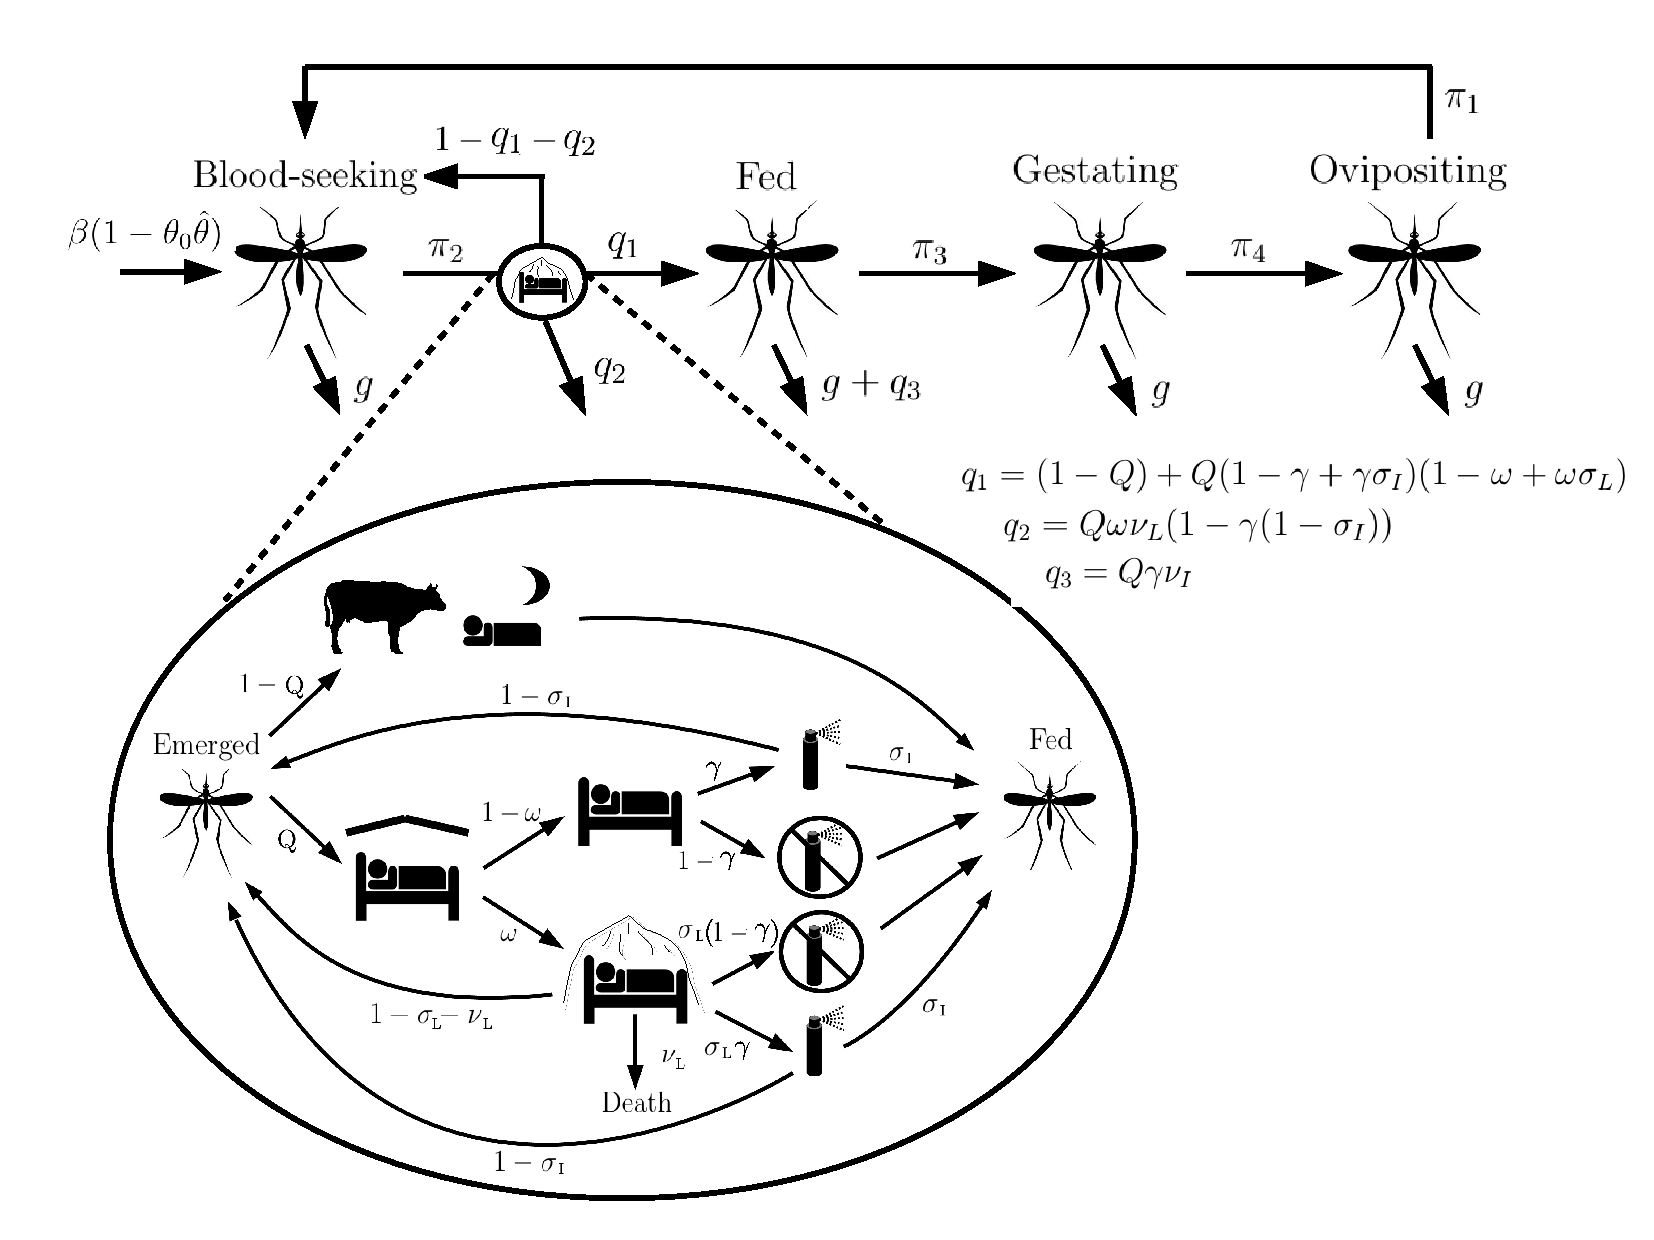
\includegraphics[height=10cm]{Project/Figures/VectorModel/Diagram_VC2019.pdf}
\caption[Gonotrophic cycle model schematic.]{Mosquito feeding dynamics. Outcomes of feeding, death and repeating are all dependant on: proportions of blood meals taken outdoors; vector control coverage; vector control efficacy parameters.}
\label{fig:diag_vec}
\end{center}
\end{figure}

\begin{table*}[t]
\caption[Mosquito parameters and sources.]{Parameters for mosquito biology and vector control (\textit{Anopheles gambiae})}% title of Table
\vspace{.1cm}
\centering % used for centering table
\begin{tabular}{|c|p{54mm}|p{48mm}|c|}% centered columns (4 columns)
\hline                        %inserts double horizontal lines
 & Definition & Value & Source \\ [0.5ex]% inserts table 
%heading
\hline                  % inserts single horizontal line
$Q$ & Fraction of blood-meals indoors & 0.9--0.95 & \cite{Killeen2000} \\
$\pi_2$ & Daily rate of feeding when blood-seeking & 1/0.68 & \cite{Killeen2000} \\
$\delta$ & Mean feeding cycle length (days) & 3 & \cite{Killeen2000} \\
$a$ & Daily rate of feeding on humans & $Q/\delta$ & \cite{Smith2012}  \\
$g$ & Natural daily death rate & 1/14 & \cite{CDCMalaria,le2007} \\
$\sigma_L$ & Probability of feeding in presence of LLINs & 6 holes: 0.121 (0.054--0.188) 80 holes: 0.318 (0.231,0.405) & \cite{Ngufor2011} \\
$\nu_L$ & Probability of pre-meal death in presence of LLINs & 6 holes: 0.495 (0.392--0.597) 80 holes: 0.373 (0.282-0.463) & \cite{Ngufor2011} \\
$\sigma_I$ & Probability of feeding in presence of IRS & 0.894 (0.856--0.931) & \cite{Ngufor2011} \\
$\nu_I$ & Probability of post-meal death in presence of IRS & 0.567 (50.7--62.6) & \cite{Ngufor2011}\\
$\hat{\theta}$ & Proportion of larvae that die from larvicidal treatment & 0.6 (0.5--0.7) & \cite{Kroeger1995}\\
$\beta$ & Adult mosquito emergence rate from larval stages & 1000-100000 (dependent on: disease and setting) & \\
[1ex]      % [1ex] adds vertical space
\hline%inserts single line
\end{tabular}
\label{table:param_vector}% is used to refer this table in the text
\end{table*}

\subsection{Generational distribution}

To gain insight into the age-structure of the vector population we consider a generational formulation of the gonotrophic cycle model, where a subscript $i$ denotes the number of times mosquitoes in a given class have completed the cycle, giving an infinite series of ODEs:
\begin{eqnarray}
\frac{dB_i}{dt} &=& \begin{cases}  \beta(1-\theta) - \pi_2(q_1+q_2)B_{i} -gB_{i} &\mbox{ if } i=0\\ \pi_1O_{i-1} - \pi_2(q_1+q_2)B_{i} -gB_{i} &\mbox{ if } i\geq 1
\end{cases}\\
\frac{dF_i}{dt} &=& \pi_2q_1B_i - \pi_3 F_i - (g+\gamma) F_i \\
\frac{dG_i}{dt} &=& \pi_3F_i - \pi_4G_i - g G_i \\
\frac{dO_i}{dt} &=& \pi_4G_i - \pi_1O_i - g O_i \,.
\label{eqn:dist}
\end{eqnarray}
Adult emergence can only occur into generation $i=0$. Using this model it is possible to calculate the \gls{parity} of the population.

It is reasonable to assume the vector population adjusts essentially instantaneously to equilibrium if vector control in a given setting is fixed, as the vector dynamics are faster than the human dynamics \cite{May1979}. We can hence derive the following relationship between sequential blood-seeking classes:
\begin{equation}
B_n^* = KB_{n-1}^*\,,
\end{equation}
where
\begin{equation}
K = \frac{\pi_1\pi_2\pi_3\pi_4q_1}{(\pi_2(q_1+q_2)+g)(\pi_3+g+q_3)(\pi_4+g)(\pi_1+g)}
\end{equation}
is a constant and $K<1$, this quantity can be interpreted as the gonotrophic cycle survival probability, or the proportion of the vectors that are gravid (have had at least one bloodmeal). As the constant term is less than unity, the difference equation can be solved to get an explicit formula, $B_n^* = K^nB_0^*$, which can be used to calculate the number of vectors in each feeding generation for initial conditions
\begin{equation}
B_0 = \frac{\beta(1-\theta)}{\pi_2(q_1+q_2)+g}\,.
\end{equation}
The proportion of the population that have completed at least one feeding cycle (are parous) is given by
\begin{equation}
1-\frac{B_0}{\sum_i B_i}\,.
\end{equation}

\subsection{Disease dynamics}

The incubation period of LF in the mosquito is approximately 8.5 days \cite{le2007,erickson2009}, and for malaria this can range from 10 to 21 days, depending on parasite species \cite{CDCMalaria}. This means infection cannot be passed on to a new host immediately after the mosquito is infected. Due to the short adult mosquito lifespans (average 10-14 days \cite{le2007}), including the infected but not yet infectious vectors in the force of infection on humans would result in a severe over-estimation when considering the proportion of infectious bites. When modelling the disease dynamics we therefore introduce an exposed class -- where a mosquito has been exposed to infection but is not yet contributing to the net force of infection on the host population. See Tables \ref{table:param_LF} and \ref{table:param_malaria} for full details of the parameter values used and their sources.

\begin{table*}[t]
\caption[LF disease parameters.]{Disease parameters for lymphatic filariasis (\textit{Wuchereria bancrofti})}% title of Table
\vspace{.1cm}
\centering % used for centering table
\begin{tabular}{|c|p{65mm}|p{35mm}|c|}% centered columns (4 columns)
\hline                        %inserts double horizontal lines
 & Definition & Value & Source \\ [0.5ex]% inserts table 
%heading
\hline                  % inserts single horizontal line
$c$ & Proportion bites on infectious humans that result in mosquito infection & 0.37 (0.15--0.6) & \cite{gambhir2008,Subramanian1998}\\
$b$ & Proportion bites from infectious mosquitoes that result in human infection & $1.43\times 10^{-4}$ & Table \ref{tab:Elim} \\
$u$ & Extrinsic incubation period in humans (days) & 285 (192--379)& \cite{Addiss2000} \\
$v$ & Intrinsic incubation period in vector (days) & 8.5 (7--10) & \cite{erickson2009} \\
$1/r$ & Worm fecund life span (years) & 6 & Table \ref{tab:Elim} \\
$x$ & Prevalence of infection in human population & & \\
$\kappa$ & Probability  vector infected after blood meal & $cx$ & \\
[1ex]      % [1ex] adds vertical space
\hline%inserts single line
\end{tabular}
\label{table:param_LF}% is used to refer this table in the text
\end{table*}

\begin{table*}[t]
\caption[Malaria disease parameters.]{Disease parameters for malaria (\textit{Plasmodium falciparum})}% title of Table
\vspace{.1cm}
\centering % used for centering table
\begin{tabular}{|c|p{74mm}|p{32mm}|c|}% centered columns (4 columns)
\hline                        %inserts double horizontal lines
 & Definition & Value & Source \\ [0.5ex]% inserts table 
%heading
\hline                  % inserts single horizontal line
$c$ & Proportion bites on infectious humans that result in mosquito infection & 0.55 (0.47-0.63) & \cite{Smith2010} \\
$b$ & Proportion bites from infectious mosquitoes that result in human infection & 0.037 (0.018-0.055) & \cite{Killeen2000} \\
$u$ & Intrinsic incubation period in humans (days) & 12 (8-23) & \cite{Boyd1937} \\
$v$ & Extrinsic incubation period in vector (days) & 10 (10-21) & \cite{Gary2001}\\
$1/r$ & Mean human infection duration (days) & 14 & \cite{CDCMalaria} \\
$x$ & Prevalence of infection in human population & varied & \\
$\kappa$ & Probability  vector infected after blood meal & $cx$ & \\
[1ex]      % [1ex] adds vertical space
\hline%inserts single line
\end{tabular}
\label{table:param_malaria}% is used to refer this table in the text
\end{table*}

We consider three disease states: susceptible ($S$), exposed ($Y$) and infectious ($Z$). Extending the ODE model (as in Eqn \ref{eqn:ODE}) to include disease requires sub-dividing each stage of the cycle into these three states, giving a new system of twelve ODEs. We assume adult emergence only occurs in the susceptible vector population. Assuming a prevalence $x$ in the human population and a probability $c$ that a vector becomes infected after biting an infectious human, then a proportion $xc$ of susceptible vectors moving from blood-seeking to fed become exposed to disease; all exposed mosquitoes can become infected, this occurs at rate $1/v$ where $v$ is the average vector incubation period. Due to timescales of infection and vector lifespan we do not consider recovery from infection. See Fig. \ref{fig:diag_vec_SEI} for a diagram of the full model dynamics.

\begin{figure}[ht]
\begin{center}
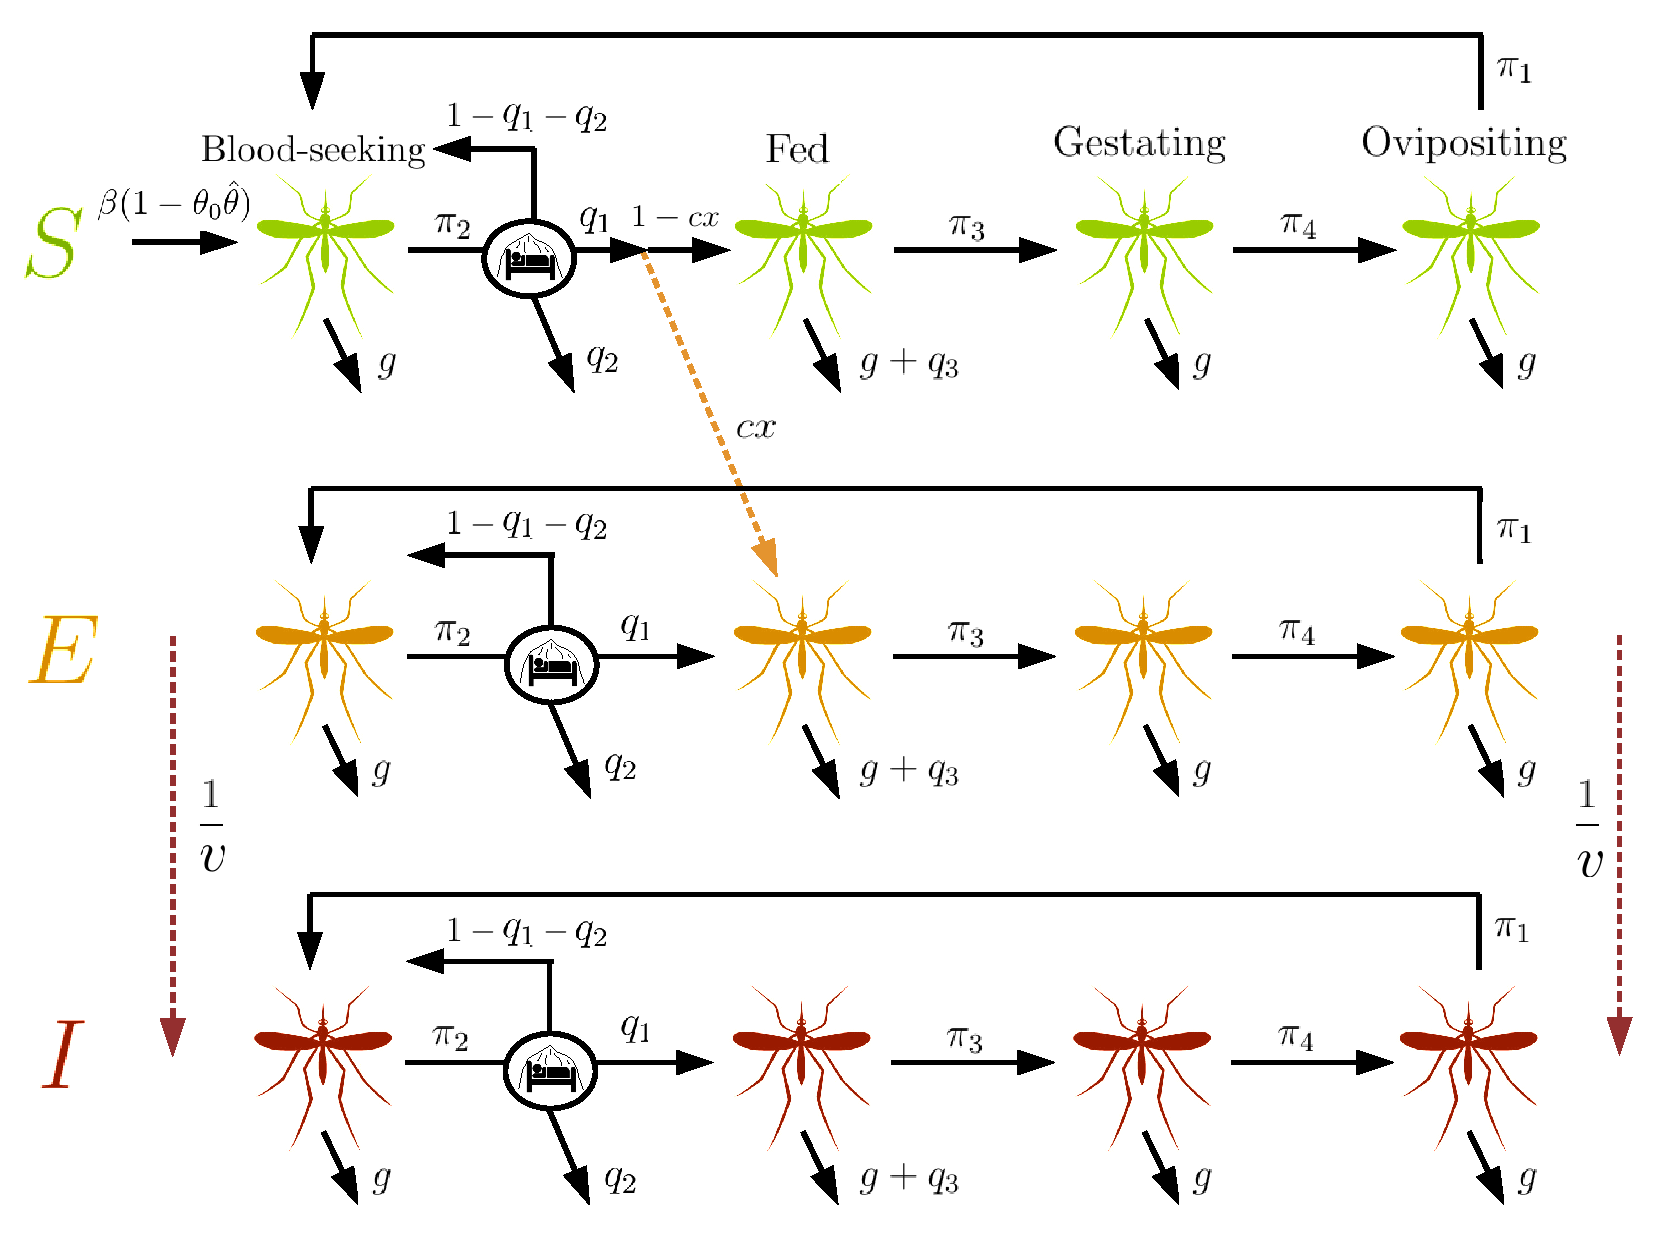
\includegraphics[height=9cm]{Project/Figures/VectorModel/Diagram_SEI2019.pdf}
\caption[Mosquito disease model schematic.]{Mosquito disease dynamics. Birth occurs in the susceptible (S) state, then during the feeding process vectors can become exposed with probability $\hat{p}=xc$ given a successful feed. Exposed (Y) vectors from all stages become infectious (Z) at rate $1/v$, where $v$ is the incubation period. Straight lines indicate transitions, diagonal lines represent deaths and dashed lines are infection events.}
\label{fig:diag_vec_SEI}
\end{center}
\end{figure}

\subsubsection{Generational distribution with disease}

%Considering instead the generational distribution model (Eqn. \ref{eqn:dist}) we can use the binomial probability, $p$, of a successful feed leading to a new vector infection to calculate the probability a mosquito is infected by the end of generation $k$:
%\begin{equation}
%p^{(k)} = \sum_{j=0}^k (1-p)^jp\,.
%\label{eqn:p}
%\end{equation}

%Assuming the vector incubation period is equivalent to approximately $n$ generations, we can calculate the equilibrium number of exposed and infected mosquitoes:
%\begin{eqnarray}
%\mbox{\# Exposed} = \sum_{i=1} E_i^* p^{(i-1)}\,,\\
%\mbox{\# Infected} = \sum_{i=n} E_i^* p^{(i-n)}\,.
%\label{eqn:numinf}
%\end{eqnarray}
%These values can be normalised to give prevalence of exposure and infection in the vector population.

%The probability of a vector in the emerged class surviving until it has successfully fed is given by
%\begin{equation}
%\mathbb{P}[\mbox{Successfully feed}] = \frac{\pi_2p_1}{\pi_2(p_1+p_2)+\delta}\,,
%\end{equation}
%which can then be used to consider the proportion of exposed mosquitoes that successfully bite and hence could go on to transmit infection. In the absence of bednets this probability is $0.980$, but increasing bednet coverage to $40\%$ results in a decrease to $0.841$, reflecting a reduction in the chance of a vector passing on infection in addition to the reduction in vector prevalence. %reword this? use better statistics - consider incubation period!

Consider instead the generational distribution model at equilibrium (Eqn. \ref{eqn:dist}), such that the number of blood-seeking vectors in generation $n$ is $K^nB_0$. It is sufficient to consider the blood-seeking class as this is the stage of the feeding cycle where vectors have potential to pick up or transmit disease through biting. If we define the binomial probability, $\hat{p}=xc$, of a successful feed leading to a new vector infection, then the probability a mosquito becomes exposed during generation $n$ is $\hat{p}^{(n)}=(1-\hat{p})^{n-1}\hat{p}$. Hence the probability a mosquito has been exposed before generation $n$ is $[1-(1-\hat{p})^n]$. Combining these gives the number of vectors in generation $n$ that are already infected:
\begin{equation}
B_0K^n[1-(1-\hat{p})^n]\,.
%C^nE_0^*(1-p)^{n-1}p\,.
\label{eqn:probinfect}
\end{equation}
The total number of diseased (exposed or infectious) vectors is given by summation across the generations;
\begin{eqnarray}
D &=& B_0\sum_{n=0}^{\infty} [K^n - K^n(1-\hat{p})^n]\\
&=& \frac{\hat{p}KB_0}{(1-K)(1-K+\hat{p}K)}\,.
%%N_D &=& \sum_{n=1}^{\infty}(1-p)^{n-1}pC^nE_0^*\\
%%&=& pE_0^*C\sum_{n=0}^{\infty}(1-p)^nC^n\\
%%&=& \frac{pE_0C}{1-C(1-p)}\,.
\end{eqnarray}

If the incubation period is assumed to be equivalent to $N$ generations (or cycles), then the probability of surviving until infectious is given by $K^N$ and can be treated as a multiplicative factor when calculating the numbers of infectious and exposed vectors:

\begin{eqnarray}
Z &=& K^ND\,,\\
Y &=& D - Z\,.
\end{eqnarray}
%If incubation period is assumed to be equivalent to $M$ generations then the probability a vector will survive at least $M$ cycles, which is given by
%\begin{equation}
%\sum_{j=M}^{\infty}C^j\,,
%\end{equation}
%can be used to calculate the number of infectious vectors:
%\begin{eqnarray}
%N_I &=& \sum_{n=1}^{\infty}\bigg(\sum_{j=M}^{\infty}C^j\bigg)p^{(n)}C^nE_0^*\\
%&=& \sum_{n=1}^{\infty}\bigg(\sum_{j=M}^{\infty}C^{j}\bigg)\bigg((1-p)^{n-1}p\bigg)\bigg(C^nE_0^*\bigg)\\
%&=& pE_0^*C\bigg(\sum_{j=0}^{\infty}C^{j+M}\bigg)\bigg(\sum_{n=1}^{\infty}(1-p)^{n-1}C^{n-1}\bigg)\\
%&=& pE_0^*C^{M+1}\bigg(\frac{1}{1-C}\bigg)\bigg(\frac{1}{1-C(1-p)}\bigg)\\
%&=&\frac{pE_0^*C^{M+1}}{(1-C)(1-C(1-p))} \,.
%\end{eqnarray}
These values can be normalised to give prevalence of exposure and infection in the vector population. Here we are fixing the range of possible EIP values in relation to the cycle length, with EIP $\in (N-1,N]$ gonotrophic cycles. This simplifies the system and allows us to derive analytical forms of the quasi-equilibrium solution of the model and a number of key transmission statistics. This assumption is not unreasonable given the comparatively narrow range of values quoted in the literature \cite{erickson2009}.

The force of infection on humans, $FoI_H$, is proportional to the number of infectious mosquitoes and the vector bite rate:
\begin{equation}
FoI_H \propto \pi_2q_1Z\,.
\end{equation}

\subsection{Transmission measures}
\label{sec:EpiMeasures}

There are a number of statistics commonly used to described transmission of vector-borne diseases. In the field, human landing catches are often used to estimate the \gls{EIR} (\acrshort{eir}), the expected number of infectious bites received by a single host each year \cite{Kilama2014}. A second measure, vectorial capacity, denotes the total number of infectious bites that would eventually arise from all the mosquitoes that bite a single infectious human on a single day \cite{Smith2010}. From the vectorial capacity we can derive the basic reproductive number, $R_0$, for vector borne diseases. This differs from the usual interpretation of $R_0$ for non-vector diseases by focusing on the vector dynamics and is also occasionally interpreted as $R_0^2$, describing the number of new infectious mosquitoes that would arise from a single infectious mosquito after one parasite generation \cite{Smith2010}. These three key measures are given by the following formulas:

\noindent Entomological innoculation rate (EIR):

\begin{equation}
E = maz \,,
\end{equation}

where $m$ is the ratio of mosquitoes to humans, $a$ is the blood feeding rate on humans, and $z$ is the fractional prevalence of infectious vectors.

\noindent Vectorial capacity:

\begin{equation}
V = \frac{ma^2p^v}{-\ln(p)} = \frac{ma^2}{g}e^{-gv} \,,
\end{equation}

where $p$ is the vector daily survival probability and $v$ is the extrinsic incubation period in the vector. Alternatively, $g$ is the instantaneous vector death rate.

\noindent Basic reproductive number:

\begin{equation}
R_0 = \frac{ma^2bc}{gr}e^{-gv} = \frac{ma^2bc}{-\ln(p)r}p^v = \frac{Vbc}{r} \,,
\end{equation}

where $b$ is the probability a bite from an infectious vector infects a human, $c$ is the probability a bite on an infectious human infects a vector, and $r$ is the human disease recovery rate.

\noindent We can calculate the total number of diseased vectors (exposed plus infectious), $D$, dependent on vector control parameters and coverage:

\begin{eqnarray}
D := Y+Z = \frac{\kappa KE_0}{(1-K)(1-K+\kappa K) \,, }\\
E_0 = \frac{\beta(1-\theta)}{\pi_2(q_1+q_2)+g} \,.
\end{eqnarray}

$E_0$ is the number of exposed vectors and $\kappa = cx$ is the probability one human blood feed results in a vector infection ($x$ is the prevalence of disease in the human population).

\noindent From this we can get the total number of infectious vectors:

\begin{equation}
Z = K^ND\,,
\end{equation}

and hence directly calculate our useful statistics. For example, the EIR is given by:

\begin{equation}
E = maK^N\bigg(\frac{\kappa KE_0}{(1-K)(1-K+\kappa K)}\bigg)\frac{1}{M}
\end{equation}

In the absence of interventions the mean feeding cycle length is,

\begin{equation}
\delta = 1/\pi_1+1/\pi_2+1/\pi_3+1/\pi_4\,,
\end{equation}

where $1/\pi_2$ is the average time to hunt and take a blood meal. IRS and larvicides won't impact hunting time, but the repelling effect of bednets will result in some vectors taking longer to move from emerged to fed.

If we assume a repelled vector begins the hunting process from scratch, then the expected time taken to successfully feed will be equal to the time taken to feed given a successful first attempt plus the expected time taken to feed scaled by the proportion of vector that repeat on any given attempt.

\begin{eqnarray}
\mathbb{E}[\mbox{Time to feed}] &=& \mathbb{E}[\mbox{Time }|\mbox{ Successful attempt}] \\
&& + \mathbb{P}[\mbox{Repeat}]\mathbb{E}[\mbox{Time to feed}]\\
\mathbb{E}[\mbox{Time to feed}] &=& \frac{1}{\pi_2} + Q\omega(1-\sigma-\nu)\mathbb{E}[\mbox{Time to feed}]\\
\mathbb{E}[\mbox{Time to feed}] &=& \frac{1}{\pi_2(1-Q\omega(1-\sigma-\nu))}
\end{eqnarray}

Now we can express overall feeding cycle length, $\delta$, in terms of bednet parameters:

\begin{eqnarray}
\delta &=& \frac{1}{\pi_2(1-Q\omega(1-\sigma-\nu))} + \frac{1}{\pi_3}+\frac{1}{\pi_4}+\frac{1}{\pi_1}\\
&=& \frac{(\pi_1\pi_3+\pi_1\pi_4+\pi_3\pi_4)\pi_2(1-Q\omega(1-\sigma-\nu))+\pi_1\pi_3\pi_4}{\pi_1\pi_2\pi_3\pi_4(1-Q\omega(1-\sigma-\nu))}
\end{eqnarray}

and the human blood feeding rate is given by:

\begin{eqnarray}
a &=& Q\bigg(\frac{1}{\pi_2(1-Q\omega(1-\sigma-\nu))} + \frac{1}{\pi_3}+\frac{1}{\pi_4}+\frac{1}{\pi_1}\bigg)^{-1}\\
&=& Q\frac{\pi_1\pi_2\pi_3\pi_4(1-Q\omega(1-\sigma-\nu))}{(\pi_1\pi_3+\pi_1\pi_4+\pi_3\pi_4)\pi_2(1-Q\omega(1-\sigma-\nu))+\pi_1\pi_3\pi_4}
\end{eqnarray}

The ratio of vectors to humans $m$, can be scaled by changes in the mosquito population ($m=M/H$), where

\begin{equation}
M = \sum_{i=0}^{\infty}E_0K^i = \frac{E_0}{1-K}
\end{equation}

and $K$ describes the probability of surviving each feeding cycle, with dependence on vector control parameters included in $E_0$ and $K$.

The death rate will depend on IRS and bednet usage. We can relate the probability of a vector surviving one feeding cycle, $K$, to a per cycle death rate $-ln(K)$, then we have

\begin{equation}
g = \frac{-ln(K)}{\delta}
\end{equation}

as the instanenous daily death rate.

Now that we have vector control dependent expressions for all relevant parameters, these can be substituted into our equations to calculate key transmission measures, such as $R_0$. In the presence of vector control measures, we relabel $R_0$ as the effective reproductive number under control, $R_e$.


%The probability of a vector in the emerged class surviving until it has successfully fed is given by
%\begin{equation}
%\mathbb{P}[\mbox{Successfully feed}] = \frac{\pi_2p_1}{\pi_2(p_1+p_2)+\delta}\,,
%\end{equation}
%which can then be used to consider the proportion of exposed mosquitoes that successfully bite and hence could go on to transmit infection. In the absence of bednets this probability is $0.980$, but increasing bednet coverage to $40\%$ results in a decrease to $0.841$, reflecting a reduction in the chance of a vector passing on infection in addition to the reduction in vector prevalence. %reword this? use better statistics - consider incubation period!
\FloatBarrier 

\subsection{Host dynamics}
\label{sec:Host}

Using the formulation laid out in the EPIFIL model \cite{Norman2000_epifil}, whilst simplifying to neglect acquired immunity and age dependency in humans, it is possible to write down an ODE model for LF host infections. Disease magnitude is described in terms of the mean worm burden ($W$) and mean mf count per 20$\mu$l of blood ($M$); acquisition of disease is dependent on the force of infection of the vector on the host population, $F_{V\rightarrow H}$, taken to be the prevalence of disease in the vector population.
\begin{eqnarray}
\frac{dW}{dt} &=& \lambda\frac{V}{H}\psi_1\psi_2\psi_3F_{V\rightarrow H} - \mu W\\
\frac{dM}{dt} &=& \alpha W - \gamma M \,.
\end{eqnarray}

Infection is described using the rate at which humans are bitten, which is given as the number of bites per mosquito per unit time, $\lambda$, multiplied by the ratio of vectors to hosts. This is combined with the proportion of L3 leaving the mosquito per bite ($\psi_1$), the proportion of these that enter the host ($\psi_2$), the proportion of L3 in the host that then develop into adult worms, and the force of infection ($F_{V\rightarrow H}$); death of adult worms occurs at rate $\mu$. Adult worms produce mf at rate $\alpha$ per 20$\mu$l of blood and mf die at rate $\gamma$.

\begin{table*}[t]
\caption[Host transmission model parameters.]{Parameter definitions and values for host model, all taken from Norman et al (2000) \cite{Norman2000_epifil}.}% title of Table
\vspace{.1cm}
\centering % used for centering table
\begin{tabular}{c l c}% centered columns (4 columns)
\hline\hline                        %inserts double horizontal lines
Parameter & Definition & Value (per month) \\ [0.5ex]% inserts table 
%heading
\hline                  % inserts single horizontal line
$\lambda$ & Number of bites per mosquito & 10 \\% inserting body of the table
$\alpha$ & Production rate of mf per worm & 2  \\
$k(M)$ & Aggregation parameter & $0.0029+0.0236\times M$ \\[1ex]      % [1ex] adds vertical space
\hline%inserts single line
\end{tabular}
\label{table:param_host}% is used to refer this table in the text
\end{table*}

Host prevalence, $P$, can then be estimated by considering the probability of an individual having greater than zero parasites per 20$\mu$l of blood:
\begin{equation}
P(M) = 1 - (1+M/k)^{-k}\,.
\label{eqn:prev}
\end{equation}

The vector model equilibrium depends on the probability one successful blood feed results in a mosquito becoming infected. Since vector dynamics are much faster than host dynamics we assume that they instantaneously adjust to quasi-equilibrium, hence we can use the current state of host infection to calculate the new vector equilibrium at each step of evaluating the host model and determine the force of infection on the host population at that point in time.

The model is hence evaluated in the following way:
\begin{enumerate}
\item The rate at which humans are bitten is fitted to the required equilibrium host prevalence in the absence of vector control, using the relationship between $M$ and prevalence given in Equation \ref{eqn:prev}.
\item The type and coverage of vector control is chosen.
\item At each step equilibrium vector prevalence is re-evaluated based on the host prevalence. 
\item The values of $W$ and $M$ are recorded at each time step; host prevalence can then be estimated if required.
\end{enumerate}

\section{Results}

In all of the following results, unless otherwise specified, we assume a 40\% human prevalence (infectious disease) to reflect a high-endemicity setting. Results for LF parameters are presented first, followed by results for malaria parameters. 

First we investigate the age-structure properties of the mosquito model and what this can tell us about transmission. We consider the age of a mosquito in terms of the number of generations, or gonotrophic cycles, it has lived through. Figure \ref{fig:propEI} shows the age-dependent probability of a vector being exposed ($E$) or infectious ($I$) by the number of gonotrophic cycles completed, in the absence of vector control. There is zero probability of being exposed or infectious in the newly emerged generation, and mosquitoes then have a probability of becoming exposed each time they feed, according to Eqn \ref{eqn:probinfect}. For LF this probability is taken to be $0.37$ if the bloodmeal is taken on an infectious host and it is assumed that it takes 3 feeding cycles to reach infectivity. For malaria these parameter are $0.4$ and 4 feeding cycles respectively, so vectors can't be infectious until they have completed their 4th feeding cycle, this means the ratio of infectious to exposed vectors is lower, with fewer infectious vectors overall. 

\begin{figure}[ht]
\begin{center}$
\begin{array}{cc}
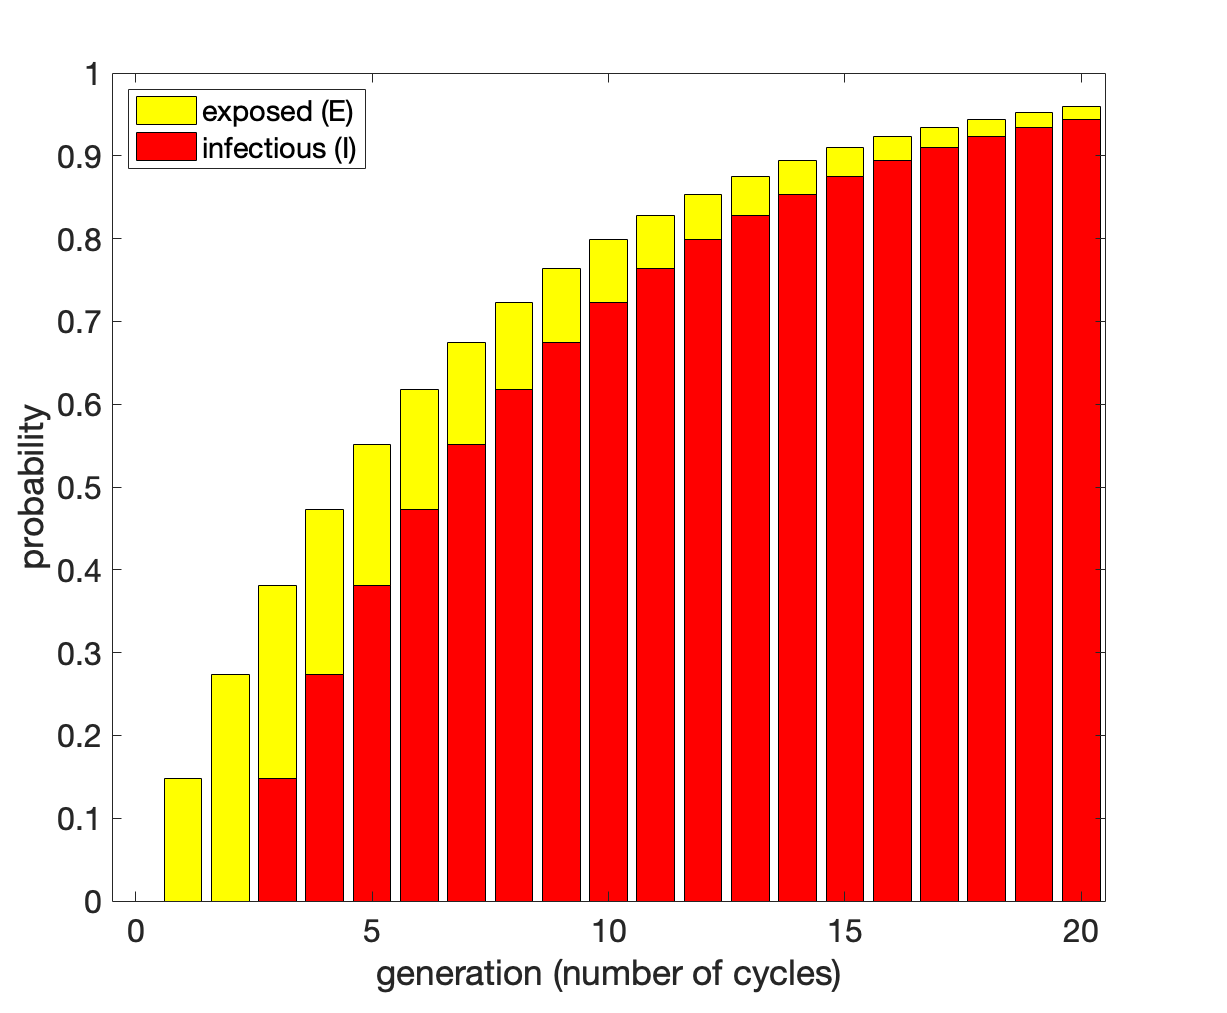
\includegraphics[height=5.8cm]{Project/Figures/VectorModel/LF/populationpropEI.png}&
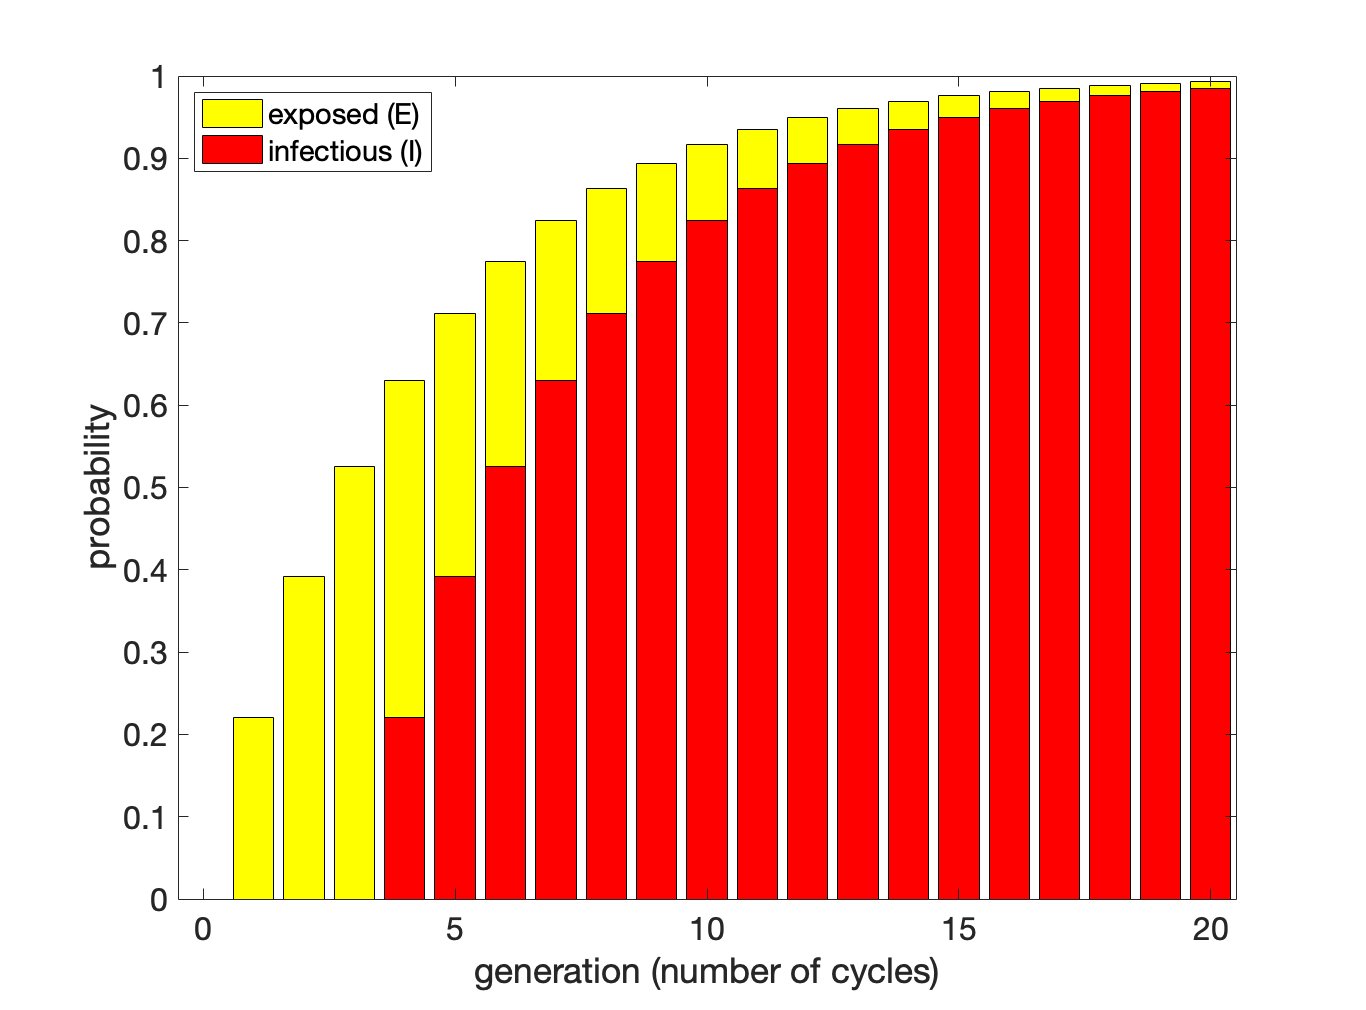
\includegraphics[height=5.8cm]{Project/Figures/VectorModel/Malaria/populationpropEI.png}
\end{array}$
\caption[Probability of exposure and infection (vector).]{Stacked bar plots showing the probability of a vector being exposed (yellow) or infectious (red) for each cycle generation. Left: For LF at 40\% host mf prevalence. Right: For malaria at 40\% host prevalence.}
\label{fig:propEI}
\end{center}
\end{figure}

\subsection{Lymphatic filariasis}

Figures \ref{fig:8controls_LF} and \ref{fig:4controls} show how the generational distribution of the mosquito population, and the presence of infection, varies according to the three different vector control interventions. We can clearly see the difference in the effects between the larvicides, which just impact the vector population size, and the other interventions, which also repel living vectors and reduce feeding. 

\begin{sidewaysfigure}[p] 
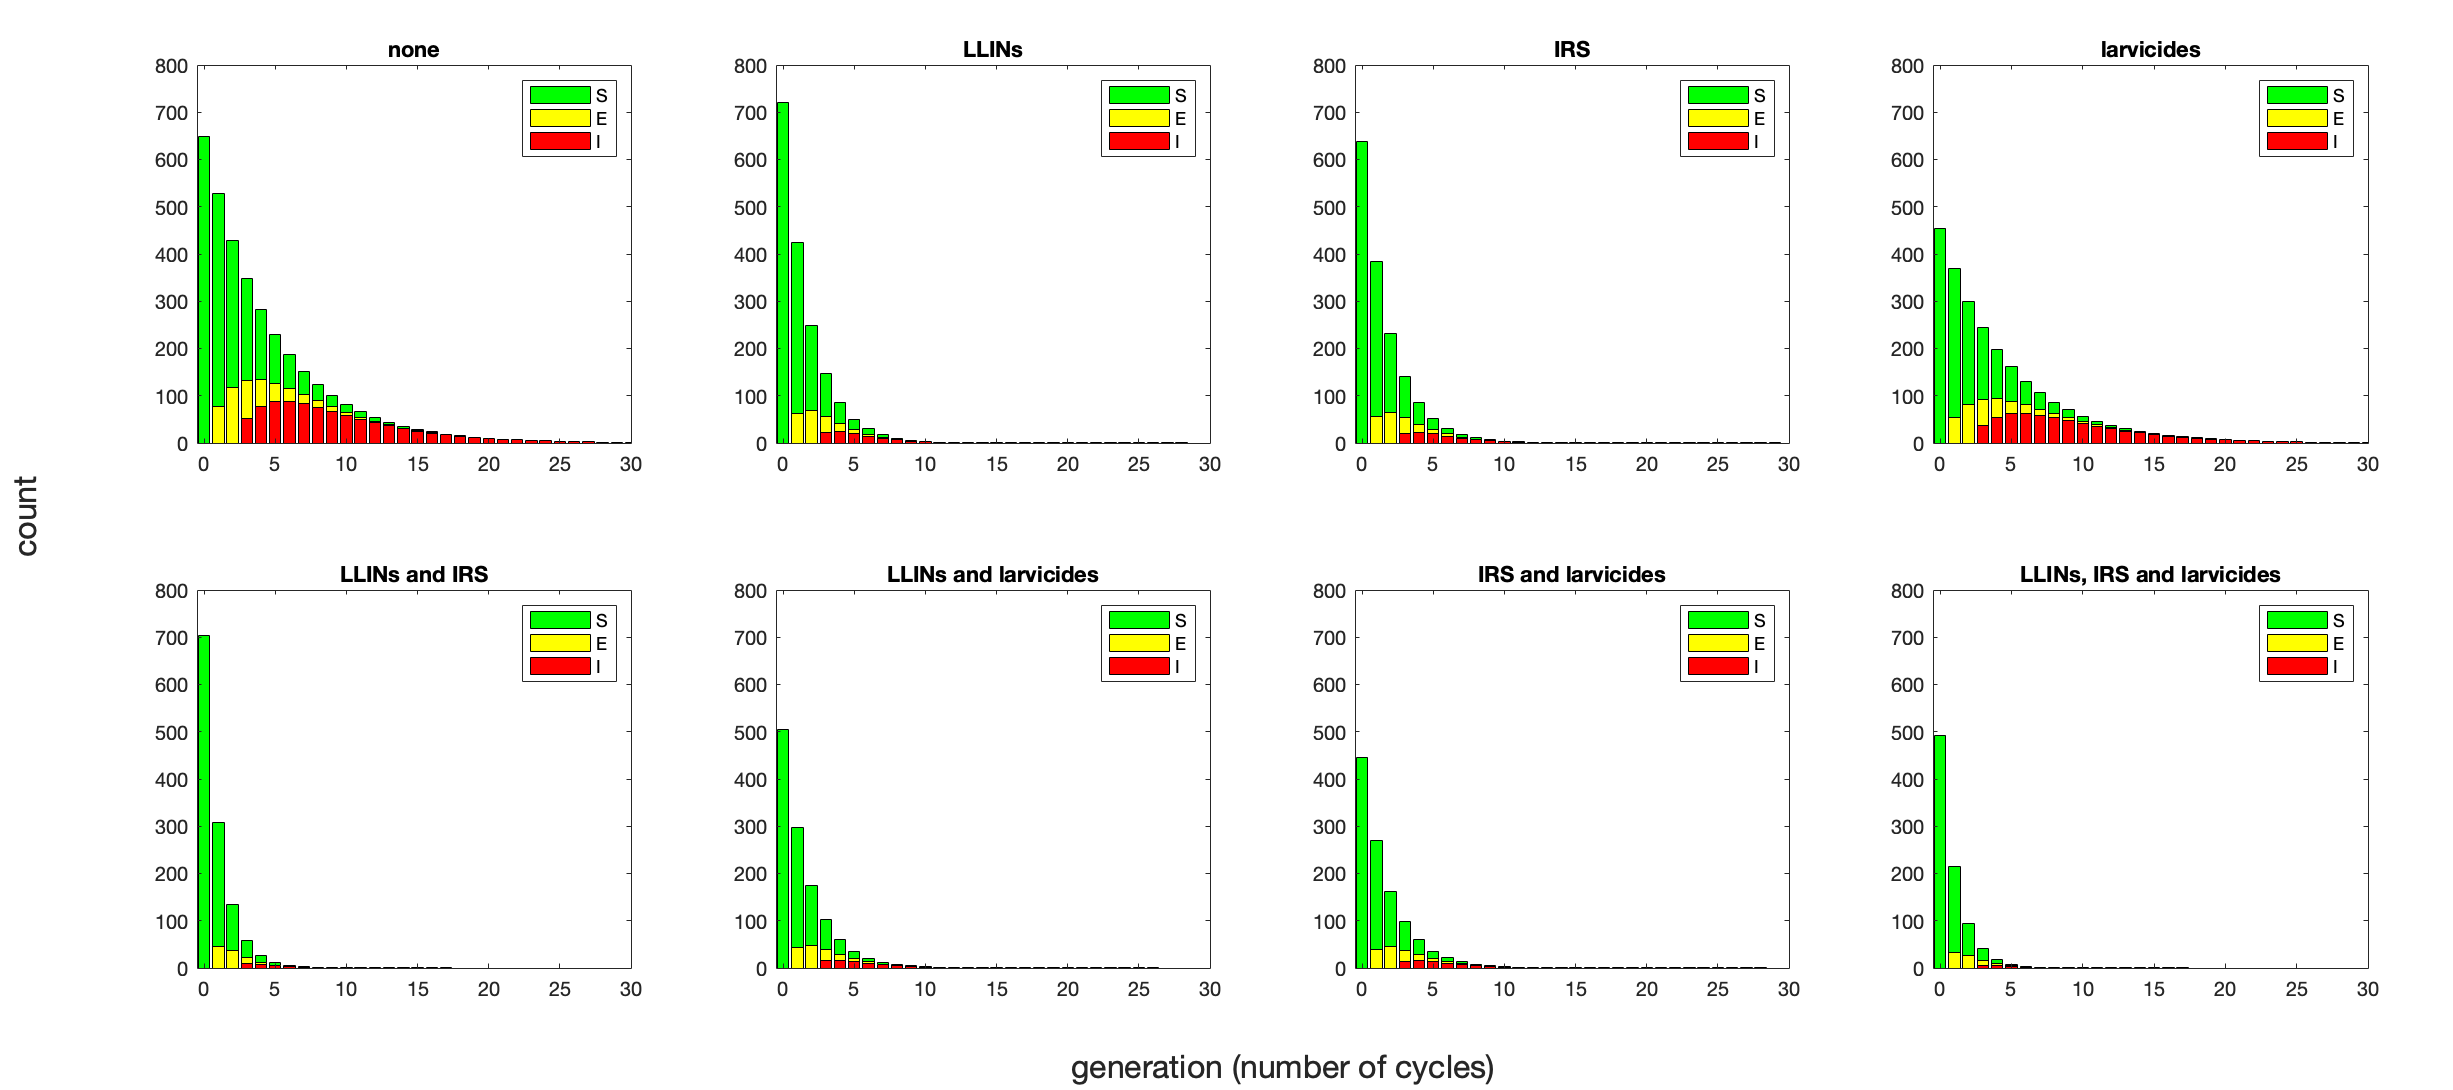
\includegraphics[height=9.7cm]{Project/Figures/VectorModel/LF/populationhist_8controls.png}
\caption[Age distribution with infection (vector count).]{Bar plots showing the age distribution of a vector population at equilibrium (total count, indexed by number of gonotrophic cycles completed) with a variety of combinations of vector control interventions. All interventions are assumed to have 50\% coverage. Bars are coloured by the proportion of vectors in each cycle generation that are susceptible (green), exposed (yellow) and infectious (red) for LF at 40\% host mf prevalence. Malaria results are presented in Figure \ref{fig:8controls_Ma}.}
\label{fig:8controls_LF}
\end{sidewaysfigure} 

LLINs, which have the highest repelling rate, cause a relative increase in the number of \gls{nulliparous} vectors (those who have taken no bloodmeals), as well as an increased death rate due to contact with insecticides. This leads to many fewer vectors in the older generations, in which infectious disease is the most prevalent and a higher frequency of mosquitoes in the younger generations, in particular generation $0$. IRS acts in a similar way, but repelling is less common and the killing effect is stronger. 

\begin{figure}[ht]
\begin{center}
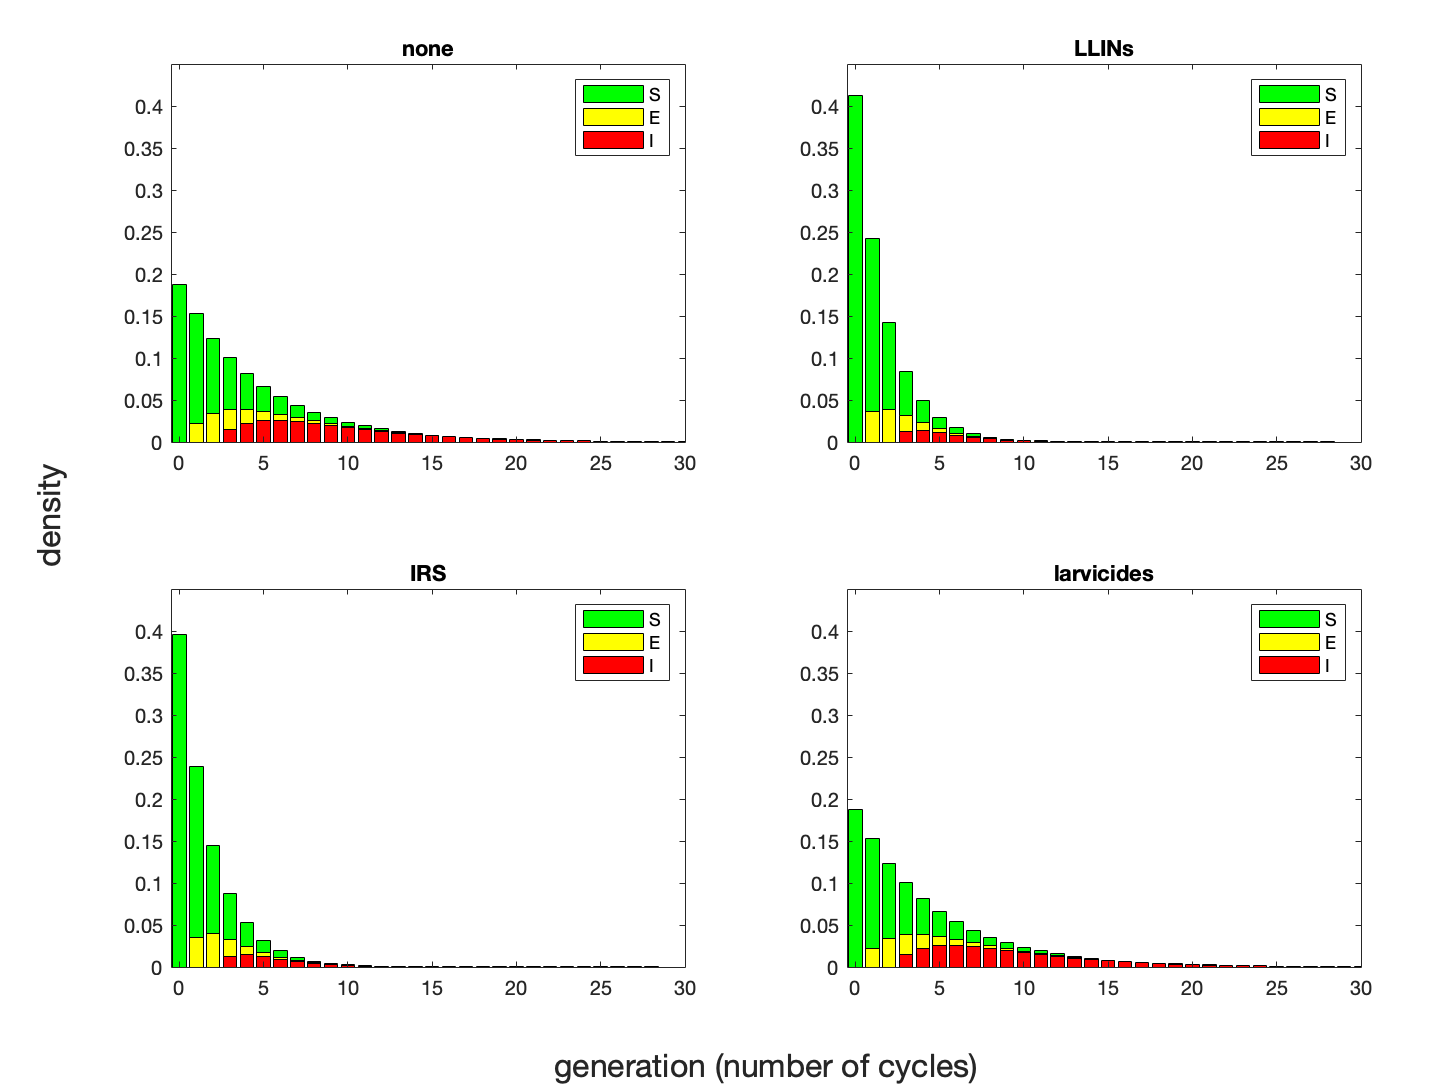
\includegraphics[height=11cm]{Project/Figures/VectorModel/LF/populationhist_4controls_density.png}
\caption[Age distribution with infection (vector density).]{Histograms showing the age distribution of a vector population (density, indexed by number of gonotrophic cycles completed) for single vector control interventions. All interventions are assumed to have 50\% coverage. Bars are coloured by the proportion of vectors in each cycle generation that are susceptible (green), exposed (yellow) and infectious (red) for LF at 40\% host mf prevalence.}
\label{fig:4controls}
\end{center}
\end{figure}

Larvicides act by reducing the emergence rate, and hence the overall population size, but as this doesn't impact adult feeding or death rates the age distribution of the population remains proportionally the same, meaning there is still a substantial infectious subset of older vectors. This is easily seen in Figure \ref{fig:4controls}, which shows the proportional distribution rather than the raw count of vectors; the larvicide histogram is an exact replica of the histogram representing no vector control measures. The LLIN and IRS histograms show more than twice the proportion of null parous vectors (around 40\% as opposed to under 20\%).

The control combinations (bottom row Figure \ref{fig:8controls_LF}) give the best outcome when adult-based control measures are combined - either IRS and LLINs or all three controls. Combining larvicides with either IRS or LLINs simply gives a scaling of the single repeating intervention effect. As the number of infectious vectors is already very low in the case of just IRS or LLIN usage, this scaling is unlikely to have an impact on transmission viability that is reflective of the level of programmatic effort required to find and treat 50\% of larval sites.

\begin{sidewaysfigure}[p] 
\begin{center}$
\begin{array}{cc}
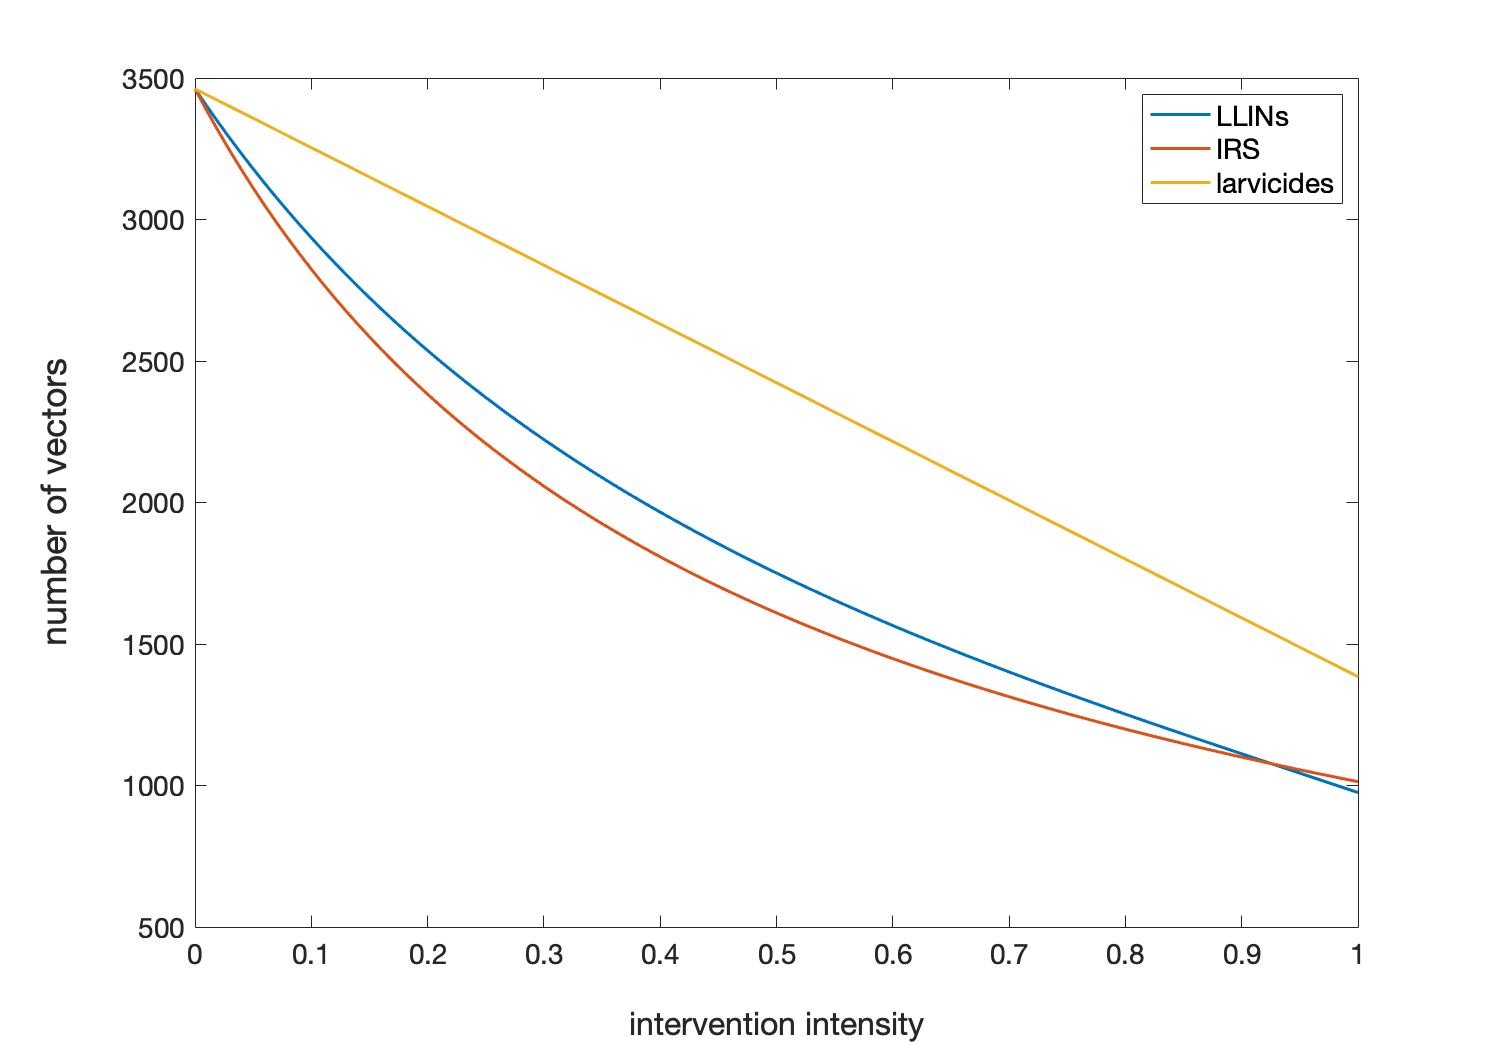
\includegraphics[height=6.7cm]{Project/Figures/VectorModel/LF/NumVec.png} & 
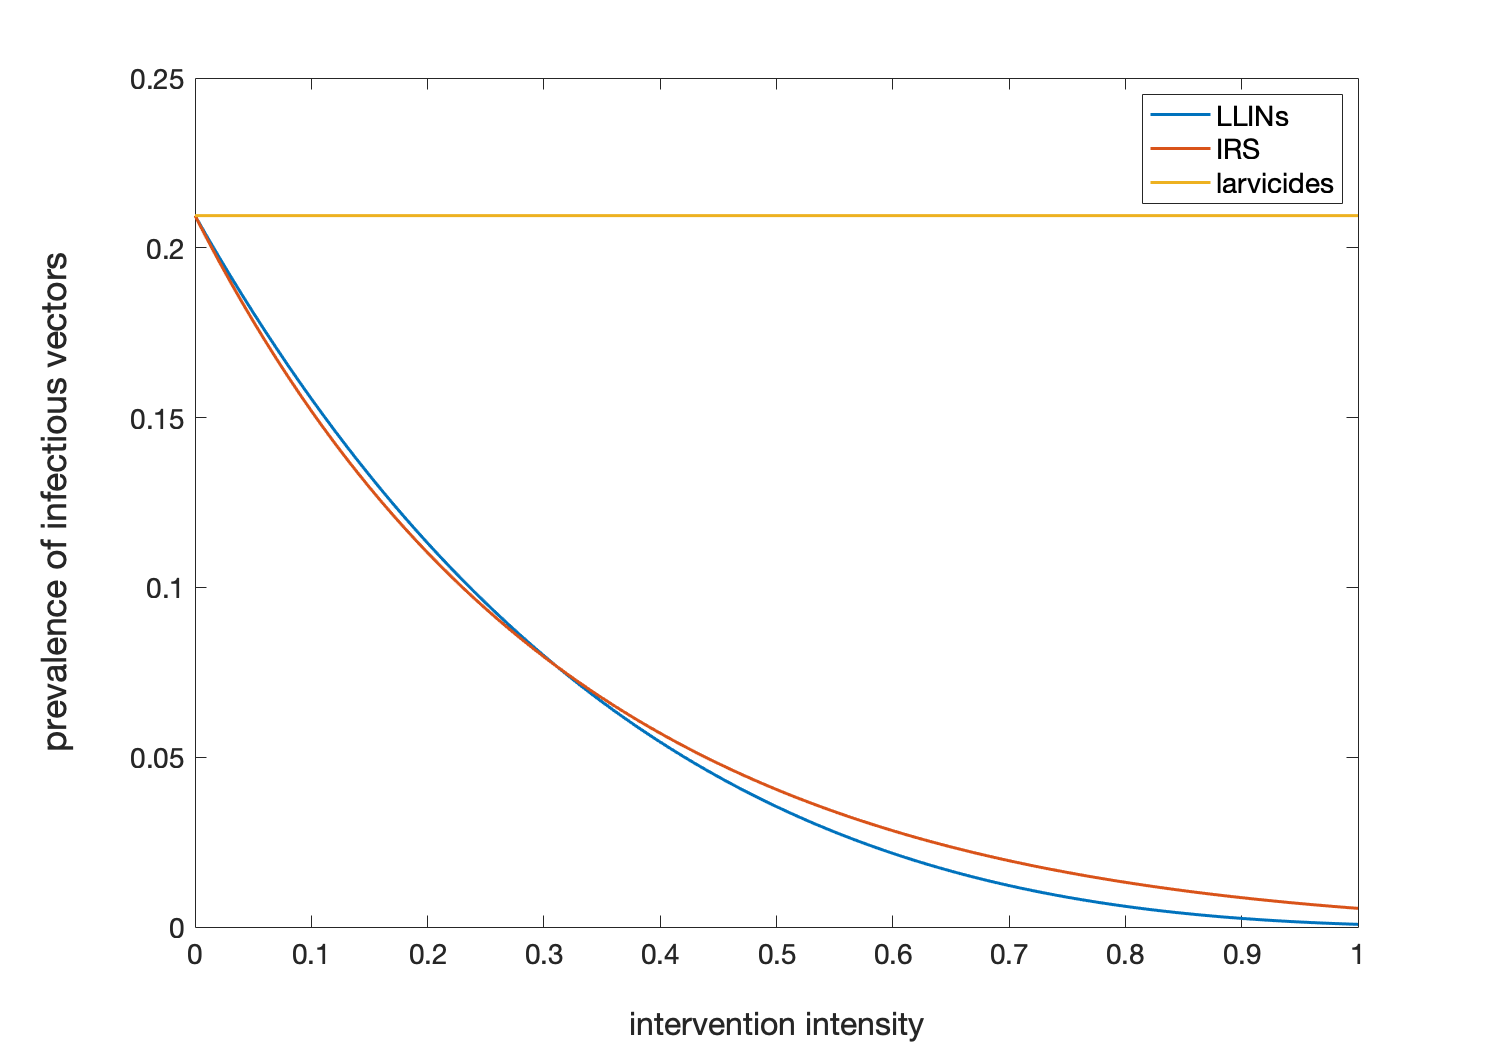
\includegraphics[height=6.7cm]{Project/Figures/VectorModel/LF/VecPrev.png} \\
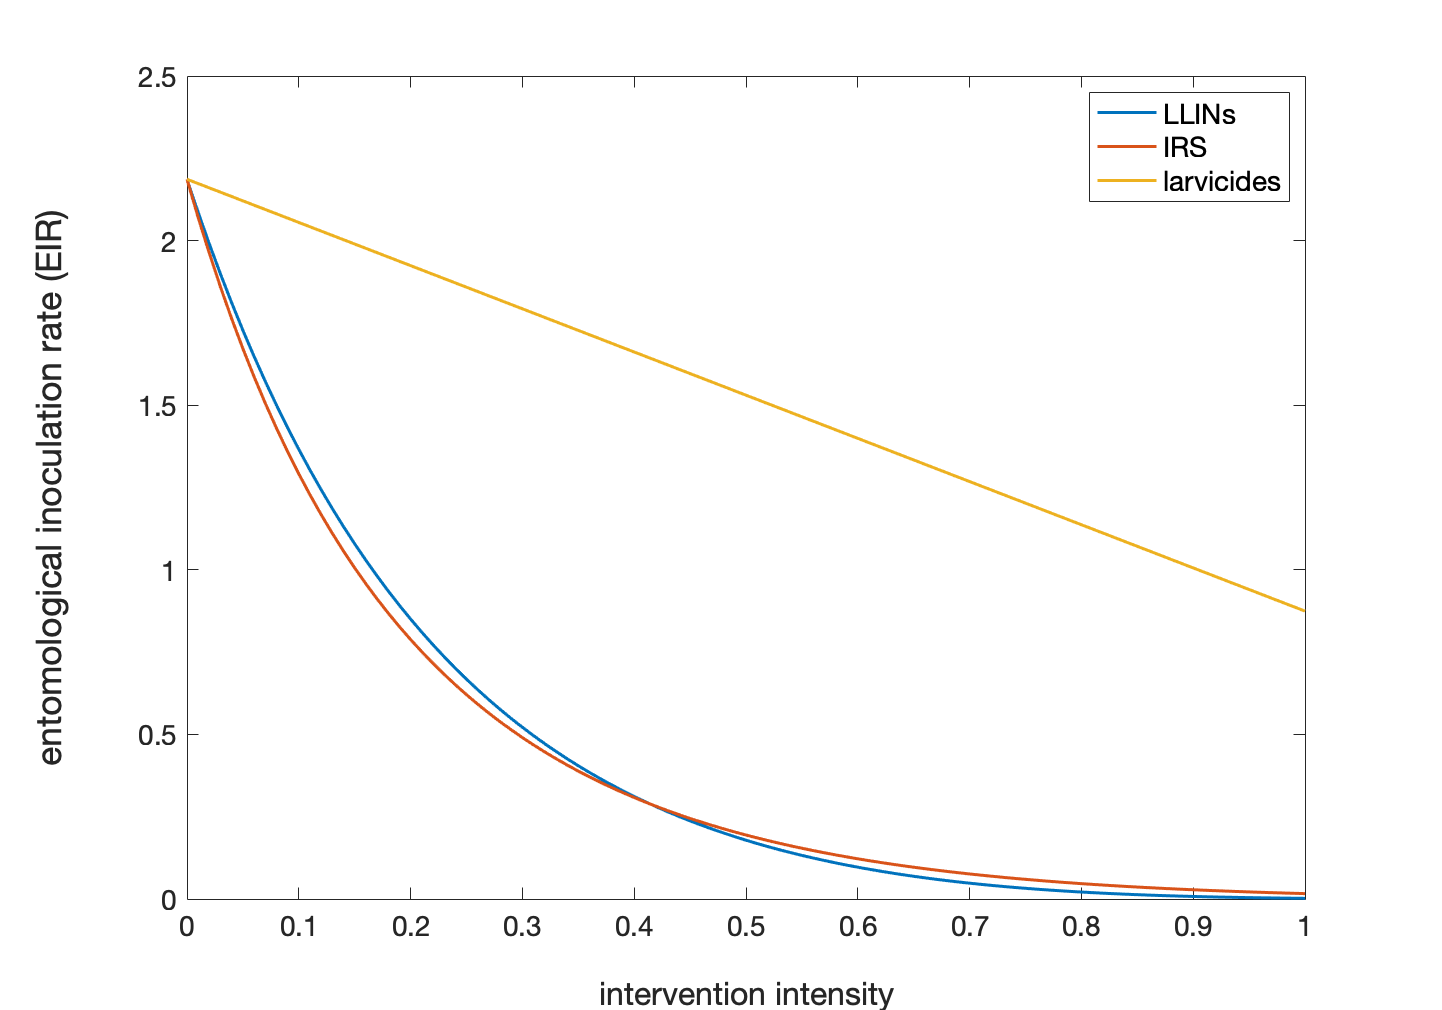
\includegraphics[height=6.7cm]{Project/Figures/VectorModel/LF/EIR.png} &
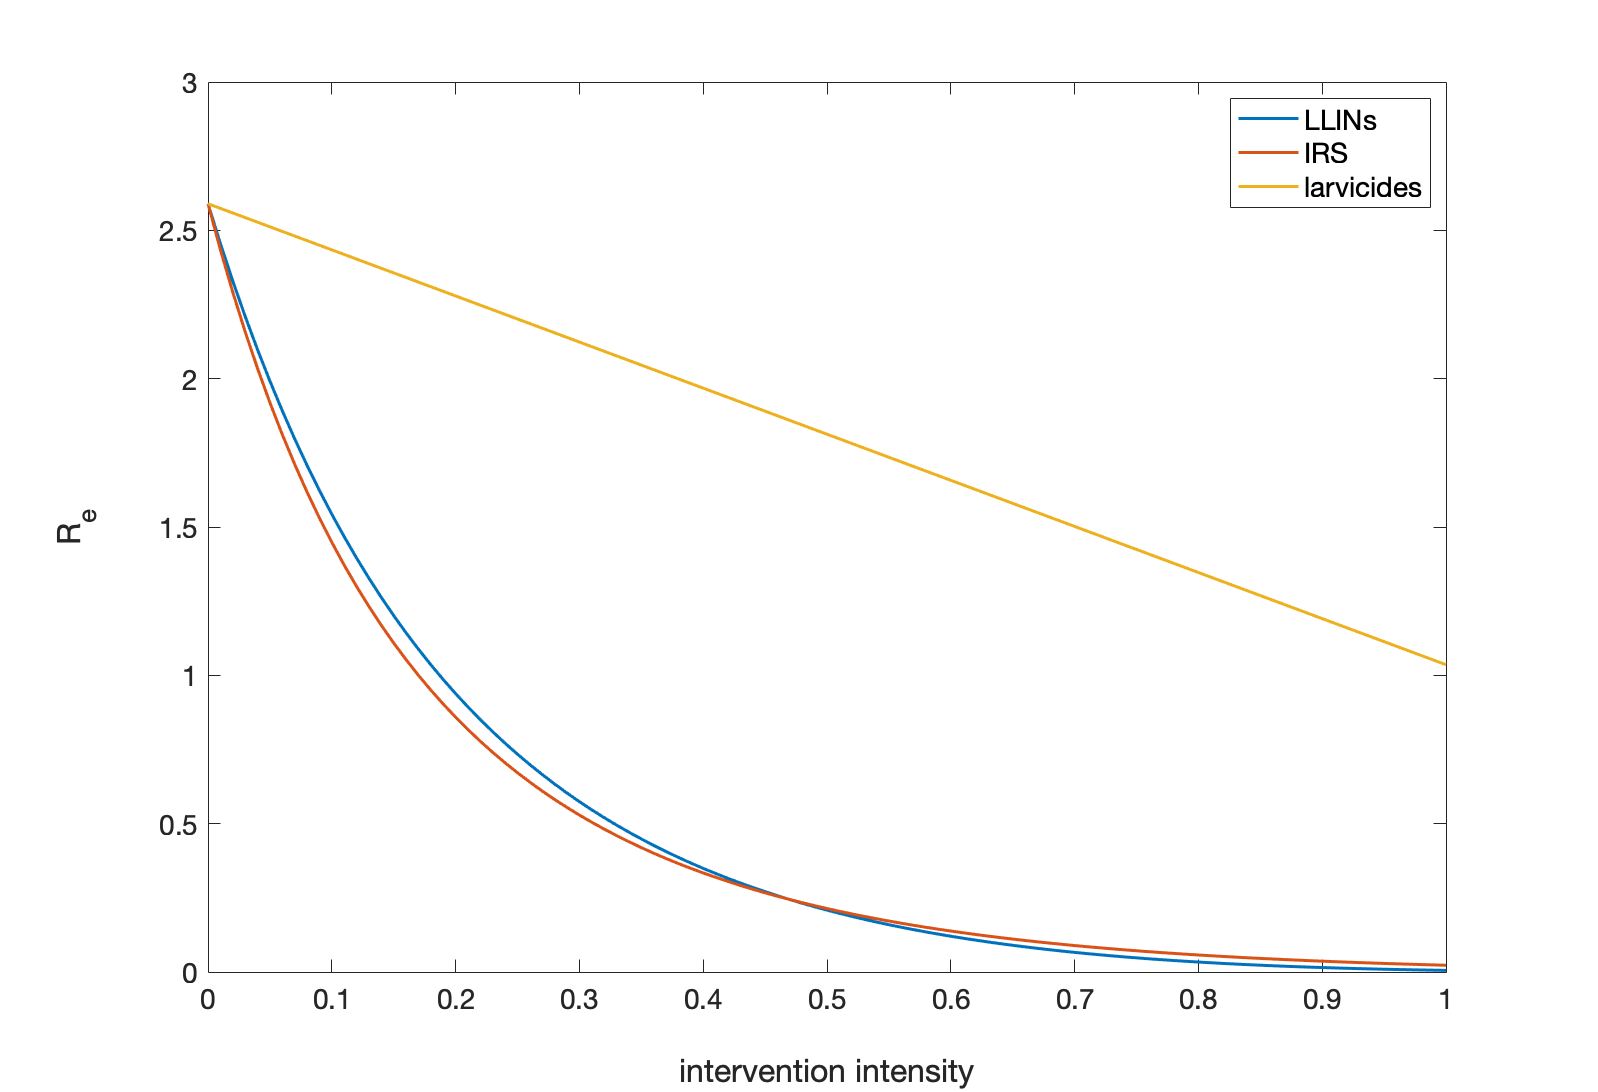
\includegraphics[height=6.7cm]{Project/Figures/VectorModel/LF/R0.png} 
\end{array}$
\caption[LF Transmission measures.]{Transmission measure comparisons for the three considered vector control interventions: LLINs (blue), IRS (red) and larvicides (yellow) from 0 to 100\% coverage. Top left: Total number of vectors in the population. Top right: Prevalence of infectious disease in vectors (not including exposed). Bottom left: Entomological inoculation rate (EIR). Bottom right: Reproductive ratio ($R_e$). For lymphatic filariasis at 40\% host mf prevalence.}
\label{fig:Epi_LF}
\end{center}
\end{sidewaysfigure} 

Having parameterised the model for LF, we can directly calculate the derived measures from Section \ref{sec:EpiMeasures} for a range of intervention intensities (see Figure \ref{fig:Epi_LF}). The emergence rate (or birth rate) of adult mosquitoes was chosen to give an $R_0$ value of approximately 2.5 in the absence of intervention \cite{Stone2014}.

In all transmission measures presented, the scale-up of larvicide coverage has the least impact and IRS and LLINs are reasonably comparable. Particularly, using larvicides doesn't decrease the prevalence of infectious vectors and has a lesser effect on the population size than either of the other two interventions. As a result, the respective decrease in key transmission measures, such as $R_e$ and the entomological inoculation rate (EIR) is only linear. Even at 100\% coverage of the adult-acting measures the vector population does not go fully extinct, and there are still very low levels of infection in the vector population. This is because IRS and LLINs are not 100\% effective at repelling or killing mosquitoes so it is still possible for a minority vectors to successfully feed, contract and potentially transmit the parasite.

The vectorial capacity is proportional to the basic reproductive number, so the results demonstrate the same effects.

\begin{sidewaysfigure}[p] 
\begin{center}$
\begin{array}{cc}
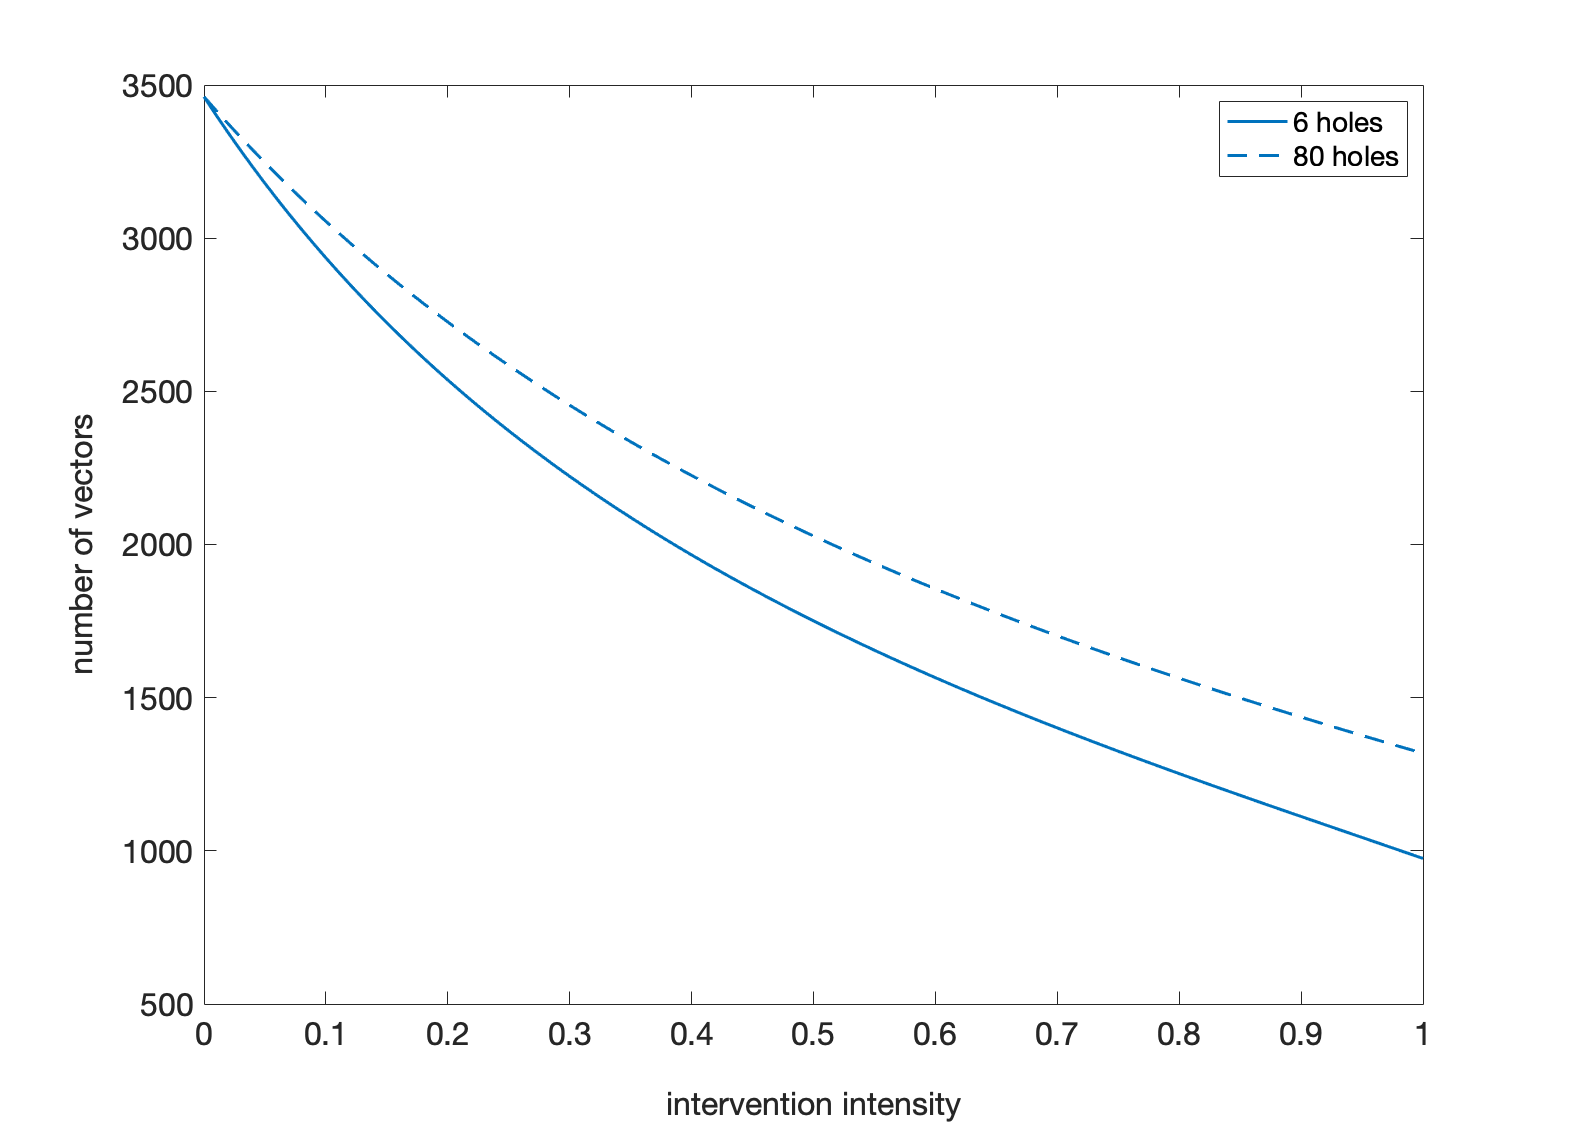
\includegraphics[height=7cm]{Project/Figures/VectorModel/LF/LLINs_holes_NumVec.png} & 
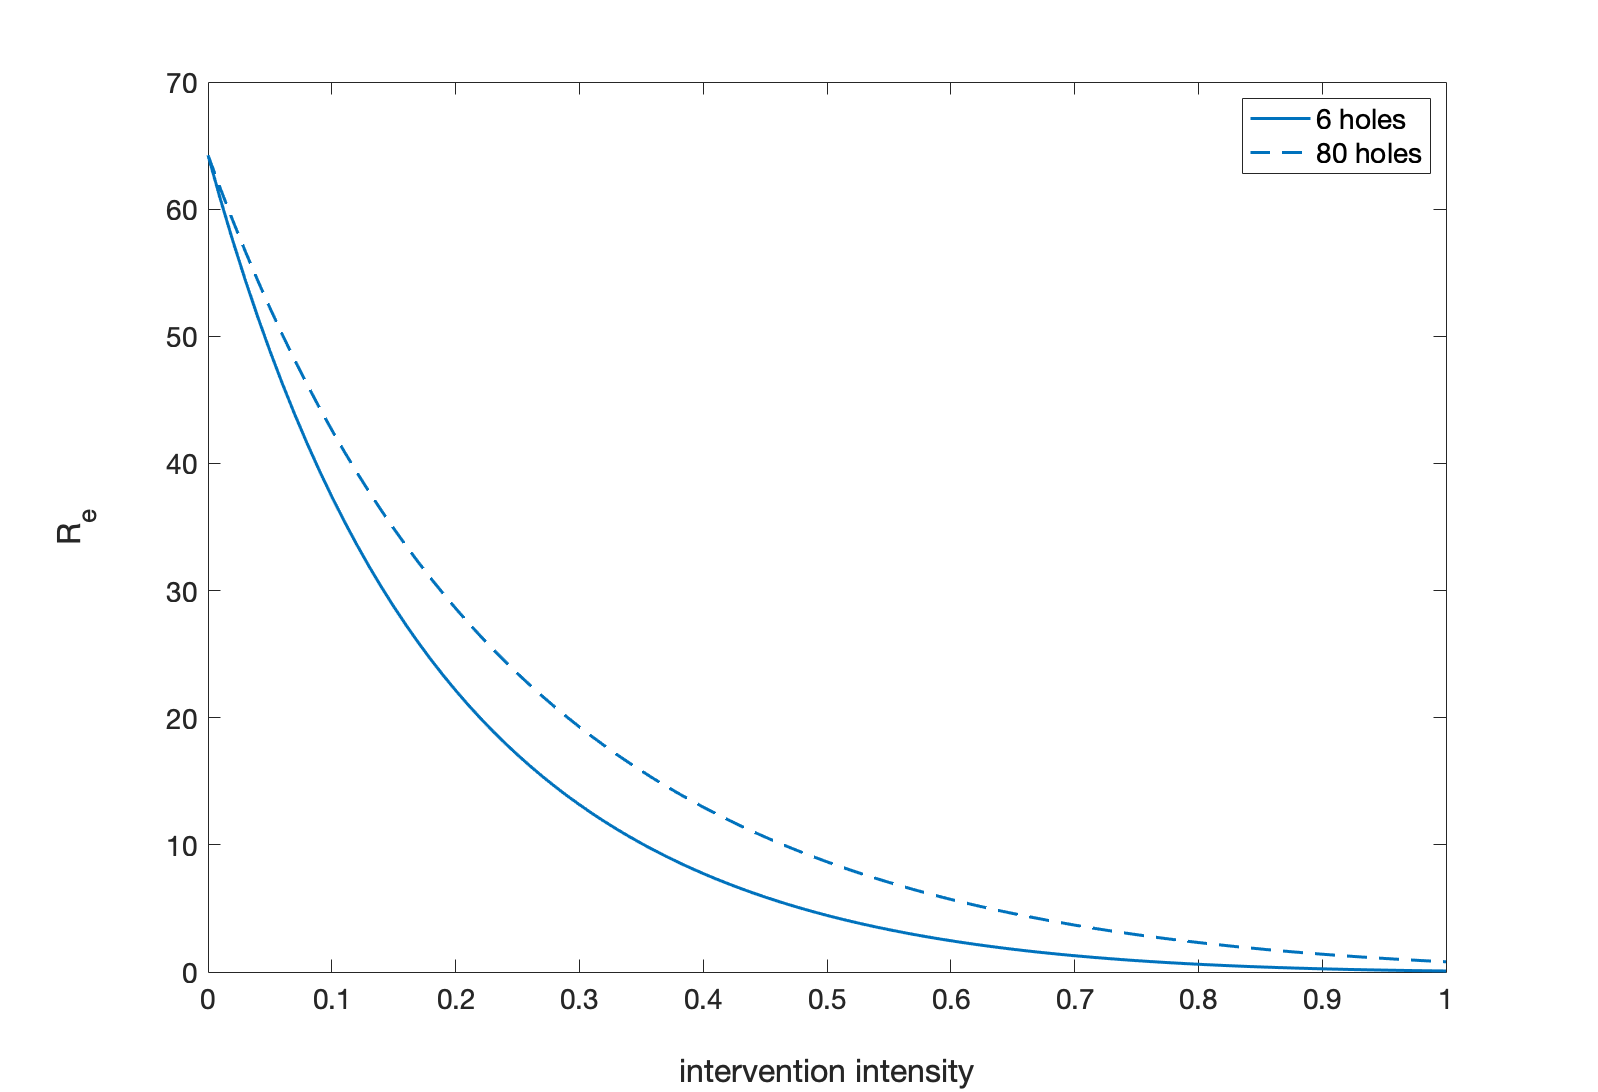
\includegraphics[height=7cm]{Project/Figures/VectorModel/LF/LLINs_holes_R0.png}
\end{array}$
\caption[LLIN integrity analysis.]{Transmission measure comparisons for LLINs of different integrity levels: 6 holes (solid) and 80 holes (dashed). Left: Total number of vectors in the population. Right: Reproductive ratio ($R_e$). For LF at 40\% host mf prevalence.}
\label{fig:holes}
\end{center}
\end{sidewaysfigure} 

In all previous plots the LLINs were assumed to be relatively new, without waning efficacy, but we can use the data presented in Section \ref{sec:VCdata} to consider how these key transmission measures change if the integrity of the nets is reduced. Figure \ref{fig:holes} shows the total number of vectors in the population and $R_e$ for a range of coverages of LLINs with 6 holes (blue, the standard assumed in previous plots) and 80 holes (red). The nets with 80 holes perform worse than the nets with 6 holes, with the biggest discrepancy in $R_e$ occurring at low-to-mid coverage levels. As the coverage level increases beyond 50\%, and the gradient flattens, the relative difference is much smaller.

\FloatBarrier

\subsection{Malaria}

Figure \ref{fig:8controls_Ma} shows how the generational distribution of the mosquito population, and the presence of infection, varies according to combinations of the three different vector control interventions (all at 50\% coverage). As with the LF results, use of larvicides has a visibly different effect to the other two interventions. As the EIP for malaria is approximately one gonotrophic cycle longer than that for LF, transmission is even more reliant on the older generations. Hence, the adult-acting interventions that shift the population distribution towards the earlier generations have an even higher impact on potential transmission.

The control combinations (bottom row Figure \ref{fig:8controls_Ma}) once again give the best outcome when adult-based control measures are combined and the addition of larvicides to any control strategy has a minimal effect on the number of infectious vectors, due to the very low number of older vectors. However, the three interventions used together is still visibly better than any other combination.

\begin{sidewaysfigure}[p] 
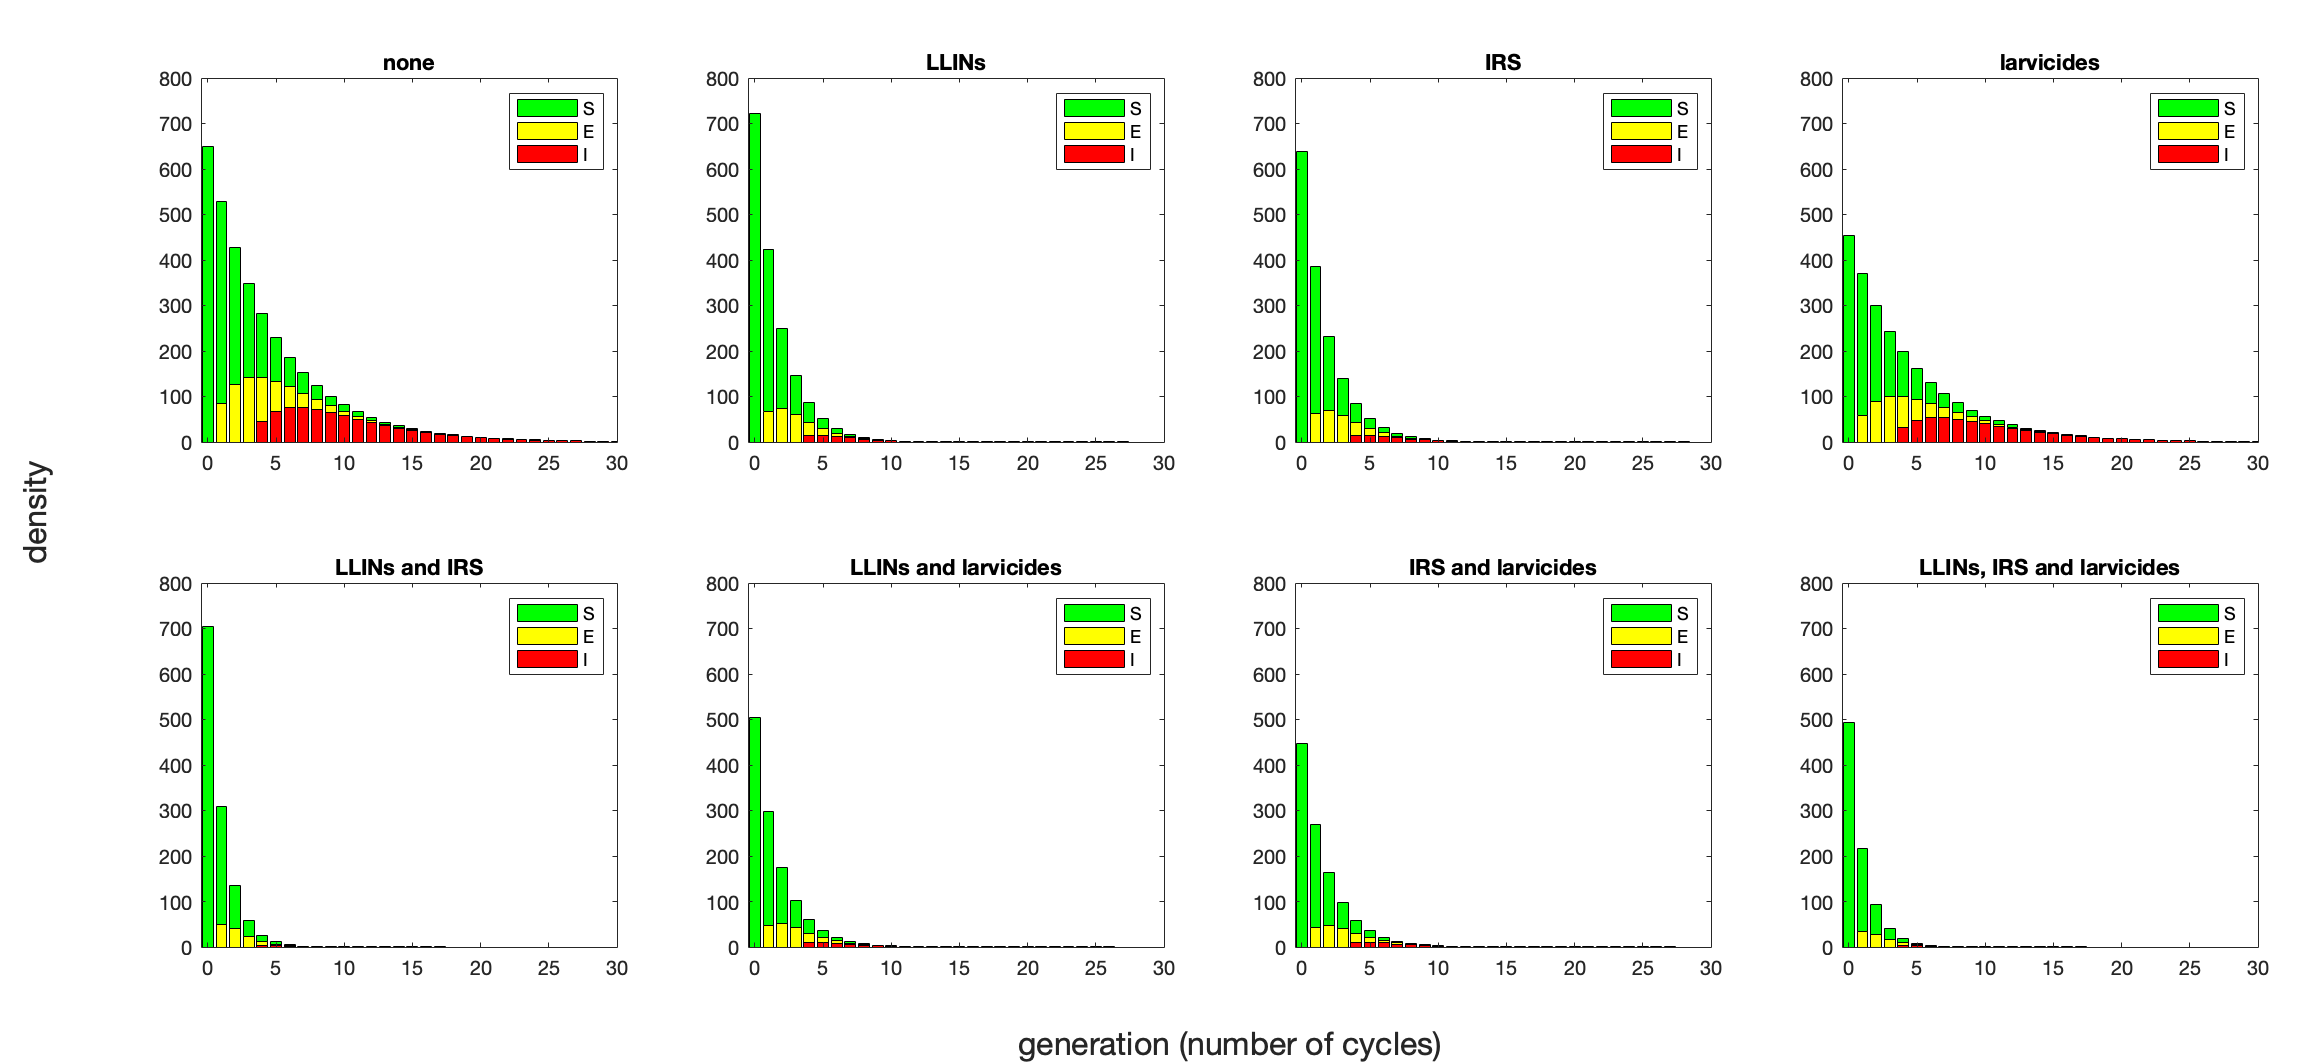
\includegraphics[height=10cm]{Project/Figures/VectorModel/Malaria/populationhist_8controls.png}
\caption[Age distribution with infection (malaria).]{Bar plots showing the age distribution of a vector population (total count, indexed by number of gonotrophic cycles completed) with a variety of combinations of vector control interventions. All interventions are assumed to have 50\% coverage. Bars are coloured by the proportion of vectors in each cycle generation that are susceptible (green), exposed (yellow) and infectious (red) for malaria at 40\% host prevalence.}
\label{fig:8controls_Ma}
\end{sidewaysfigure} 

\begin{sidewaysfigure}[p] 
\begin{center}$
\begin{array}{cc}
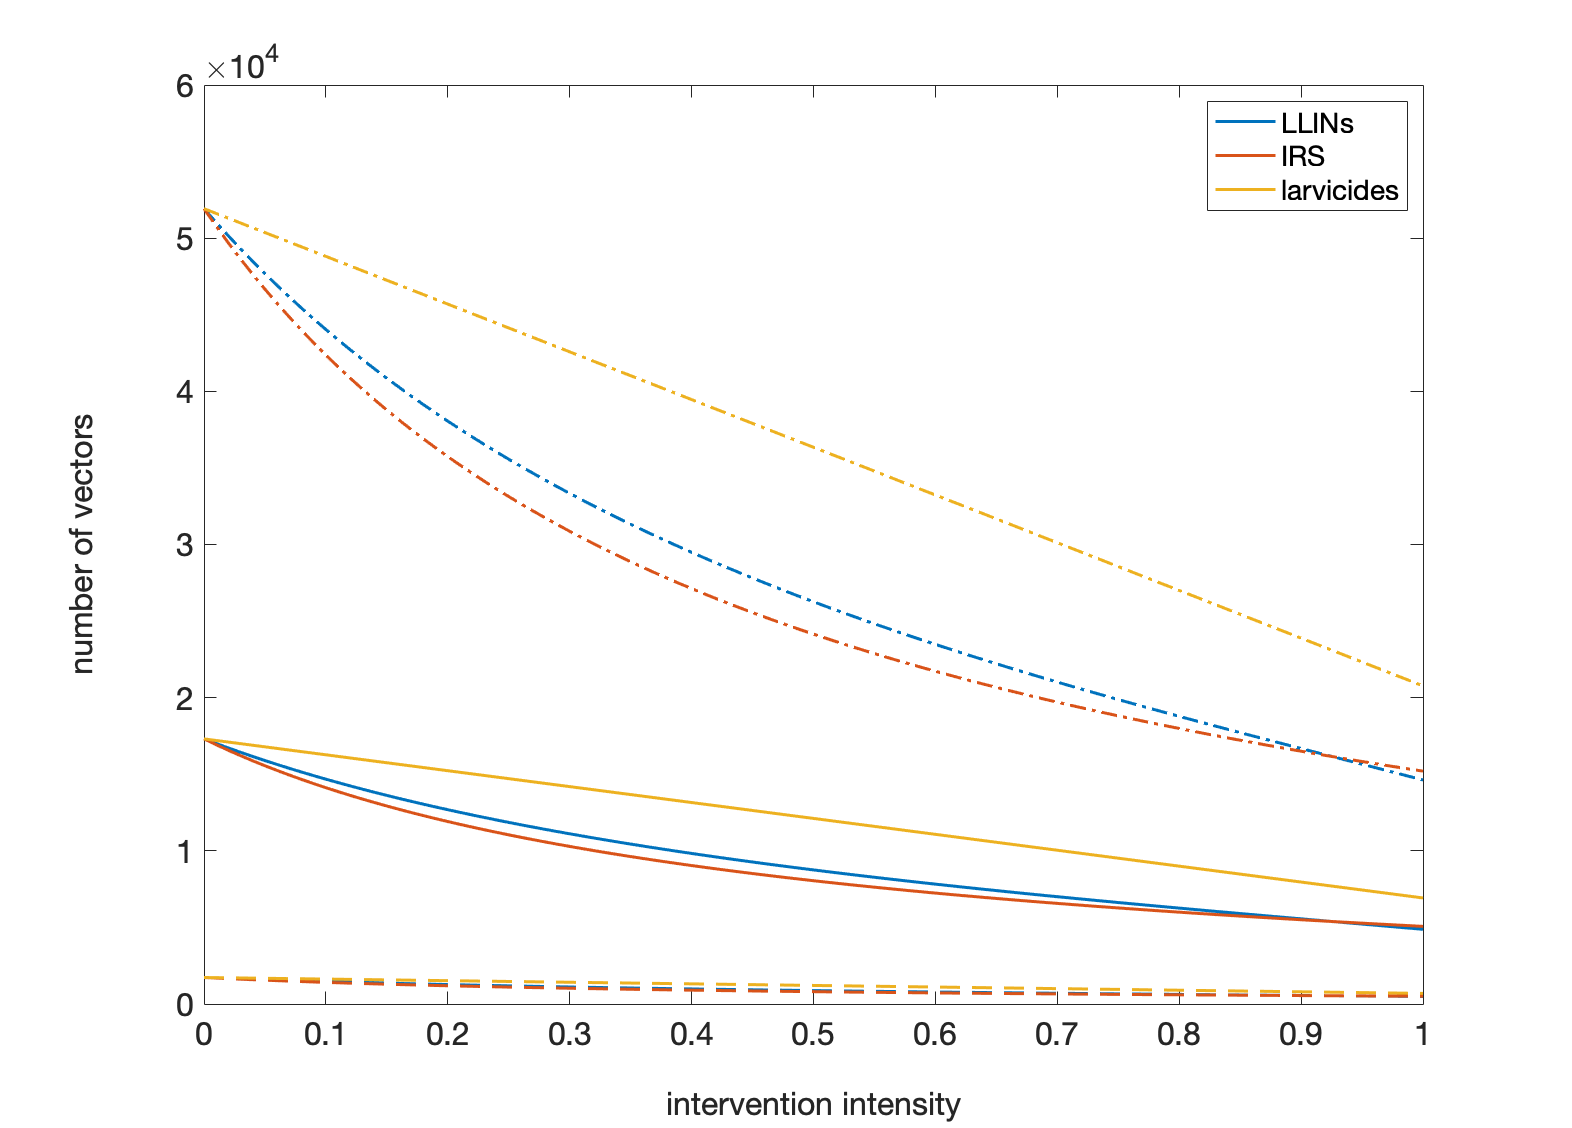
\includegraphics[height=6.7cm]{Project/Figures/VectorModel/Malaria/NumVec_lowmidhigh_new.png} & 
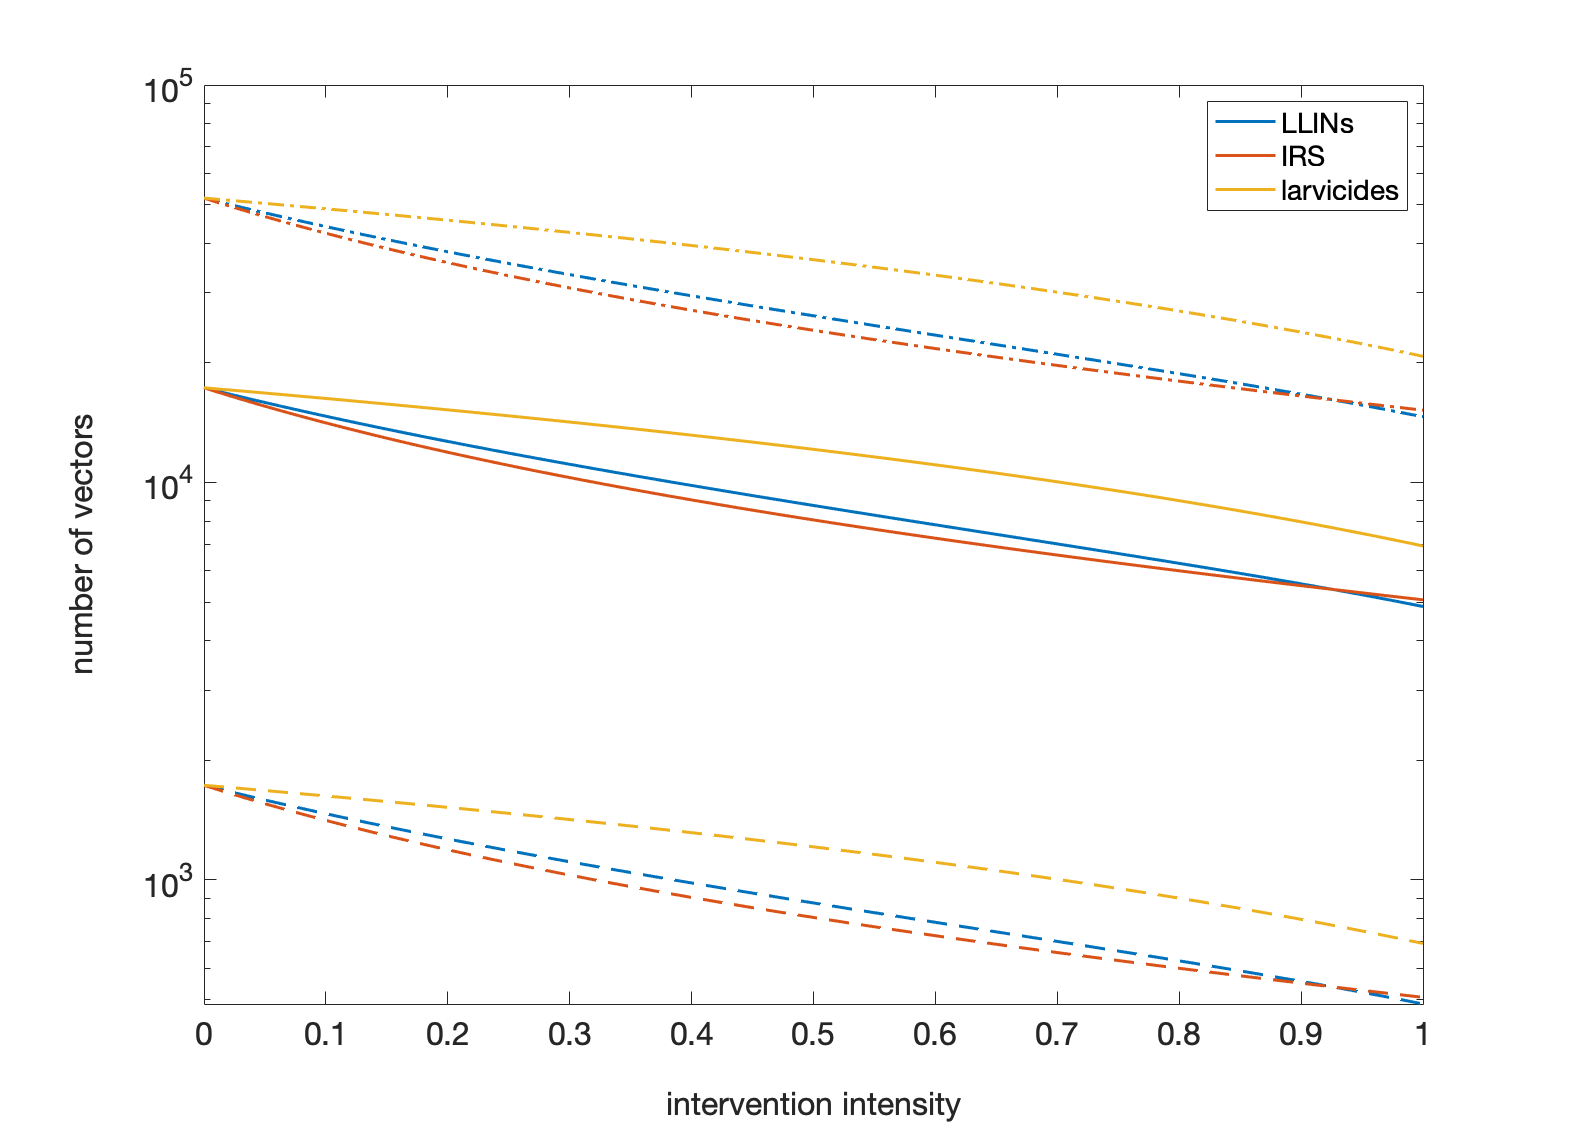
\includegraphics[height=6.7cm]{Project/Figures/VectorModel/Malaria/NumVec_lowmidhigh_log_new.png} \\
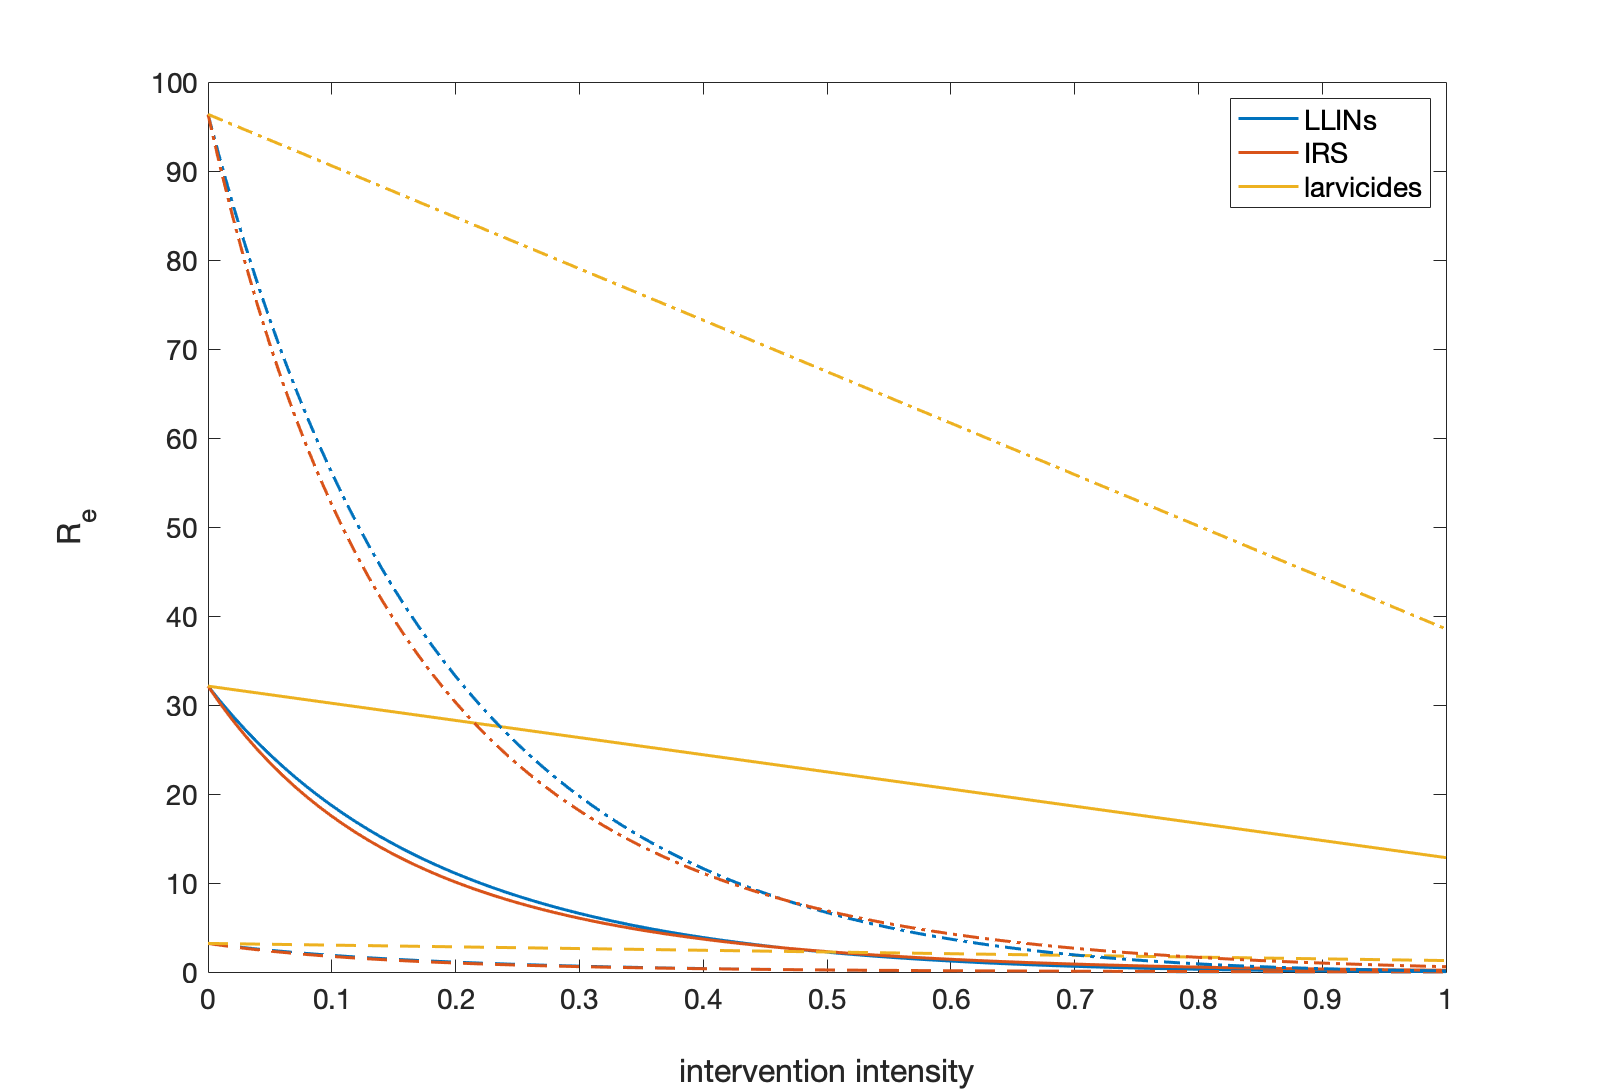
\includegraphics[height=6.7cm]{Project/Figures/VectorModel/Malaria/R0_lowmidhigh_new.png} &
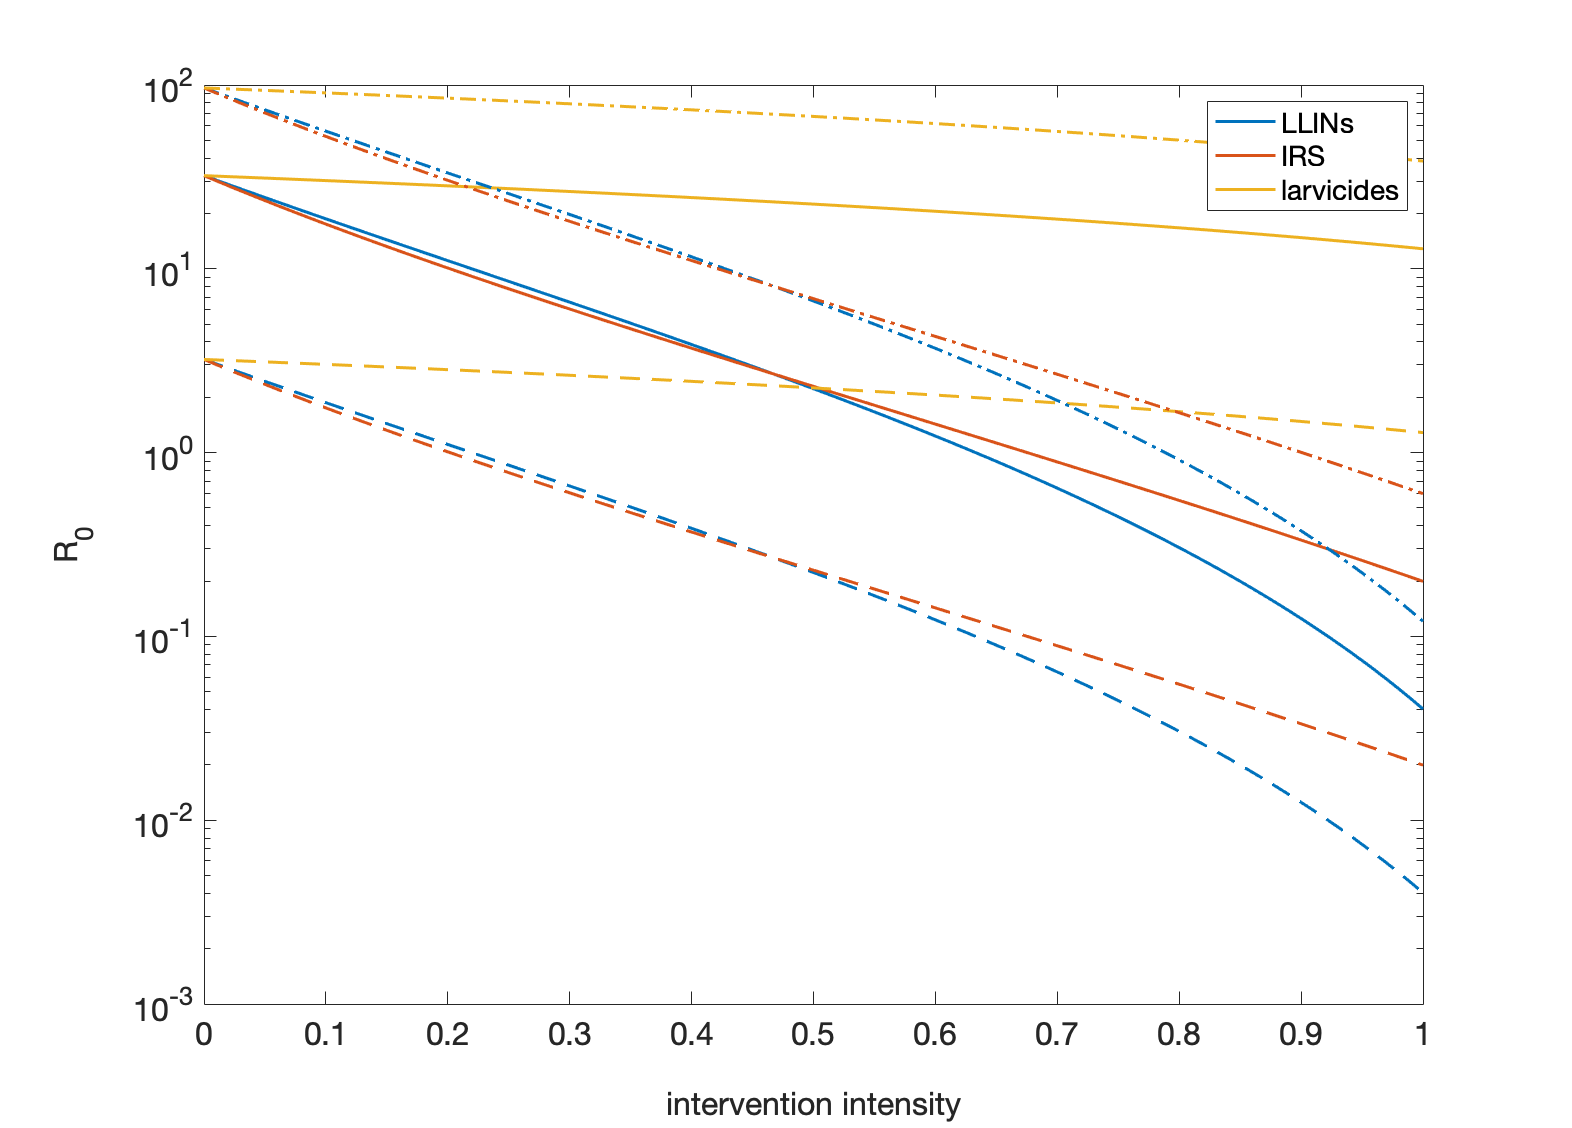
\includegraphics[height=6.7cm]{Project/Figures/VectorModel/Malaria/R0_lowmidhigh_log_new.png} 
\end{array}$
\caption[Malaria transmission measures.]{Transmission measure comparisons for the three considered vector control interventions: LLINs (blue), IRS (red) and larvicides (yellow) from 0 to 100\% coverage for high (dot-dashed), medium (solid) and low (dashed) transmission levels. Top left: Total number of vectors in the population. Top right: Total number of vectors in the population (log-scale y axis). Bottom left: Reproductive ratio ($R_e$). Bottom right: Reproductive ratio $R_e$ (log-scale y axis). For malaria at 40\% host prevalence.}
\label{fig:EpiMeasures_Ma}
\end{center}
\end{sidewaysfigure} 

When calculating the epidemiological measures, such as the EIR, for malaria it is difficult to set a fixed transmission level that is representative of malaria endemic settings, as estimates of $R_0$ in the literature vary dramatically with one review study reporting estimated values of $R_0$ ranging between one and more than 3,000 \cite{Smith2007}. Another study gives ranges between 1.3 for the lowest endemicity regions to 175.6 for the highest \cite{Gething2010}. As a result, in Figure \ref{fig:EpiMeasures_Ma} we have considered three different scenarios: high transmission (red, $R_0=400$), medium transmission (blue, $R_0=40$) and low transmission (green, $R_0=4)$. Log-scale plots are presented alongside the standard linear-scale plots to enable easier comparison between control measures for the medium and low transmission settings.

As before, the larvicides have much less impact on both the total number of vectors and the basic reproductive number than the other two adult-acting interventions. However, the log plot of the basic reproductive number shows an interesting deviation between LLINs and IRS at the higher levels of coverage that isn't visible on the linear-scale plot. This is due to the very low rate of successful feeding in the presence of LLINs (0.121), which results in much less successful feeding at high coverage due to a saturation of LLIN usage. IRS allows a higher feeding proportion (0.894 with 57\% dying post-feed) this means over 50\% of vectors seeking a blood meal will successfully feed and survive, even if every house is sprayed.

\begin{figure}[ht]
\begin{center}
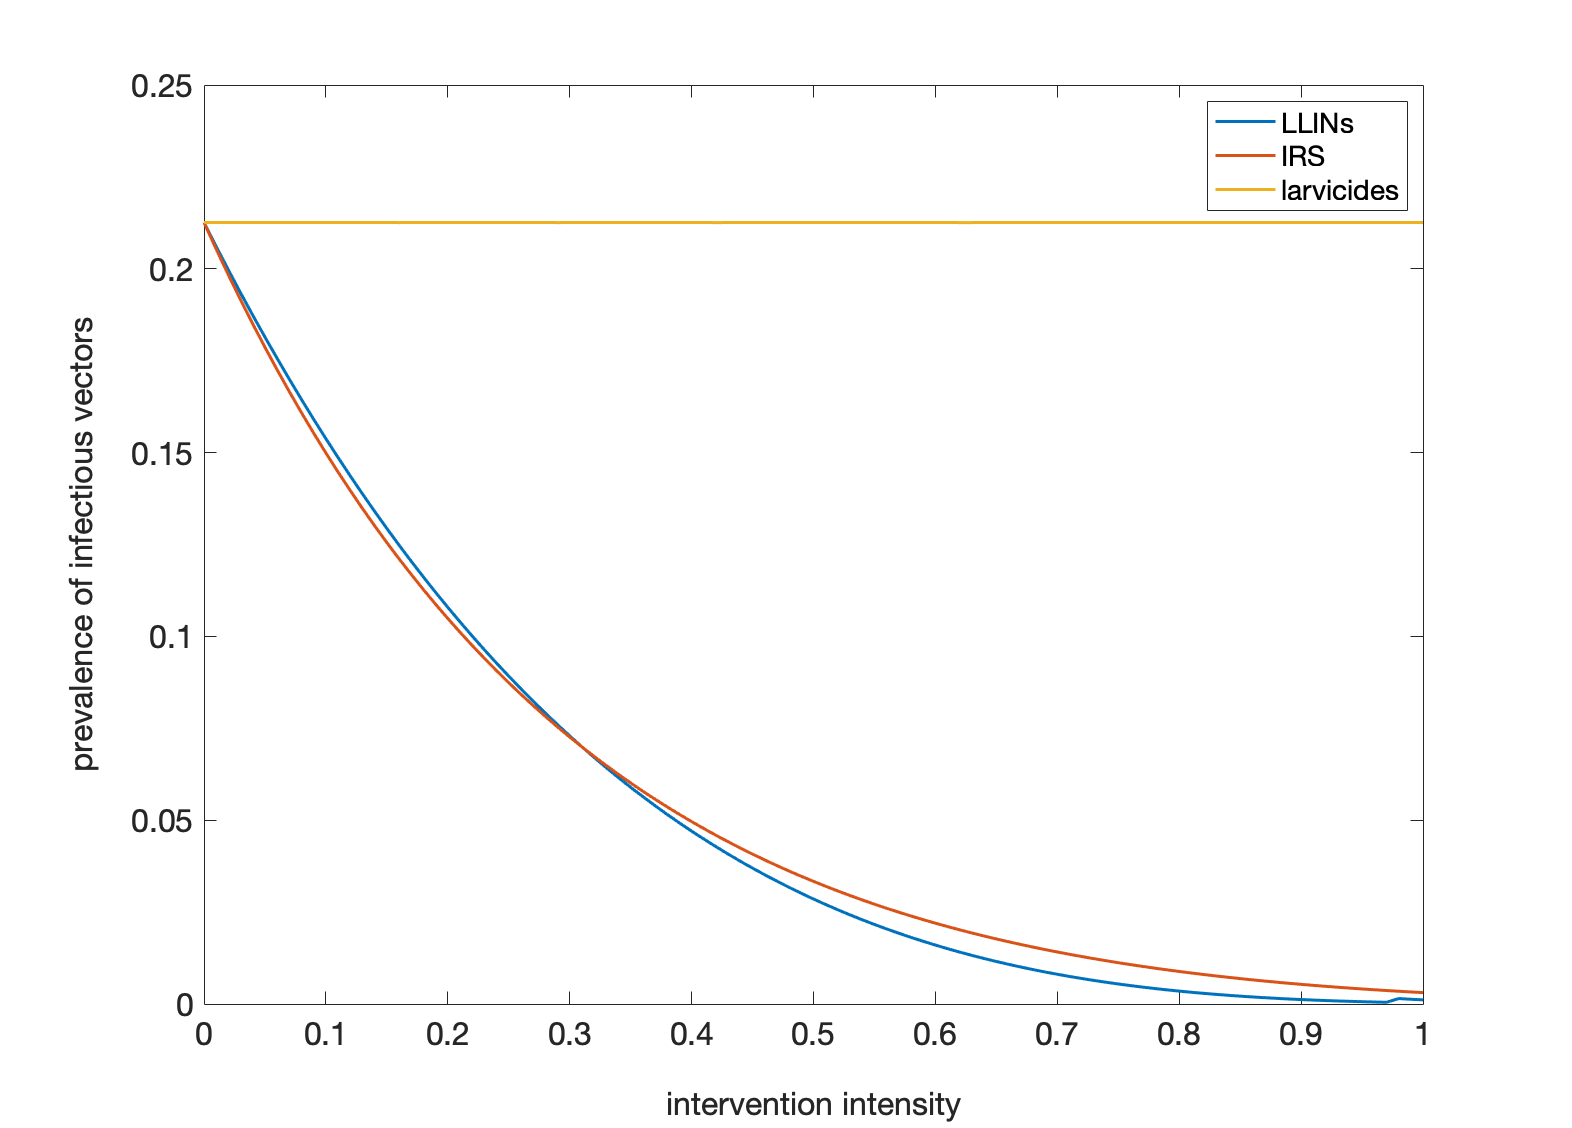
\includegraphics[height=8cm]{Project/Figures/VectorModel/Malaria/VecPrev_lowmidhigh_new.png}
\caption[Vector prevalence (malaria).]{Infectious vector prevalence comparison for the three considered vector control interventions: LLINs (blue), IRS (red) and larvicides (yellow) from 0 to 100\% coverage. For malaria at 40\% host prevalence.}
\label{fig:VecPrev_Ma}
\end{center}
\end{figure}

Figure \ref{fig:VecPrev_Ma} shows the prevalence of infectious vectors according to intervention intensity. As this is a proportional measure it is the same for all three of the low, medium and high transmission scenarios. The plot once again echoes the LF results, with larvicide coverage making no difference to vector prevalence and IRS and LLINs appearing relatively comparable throughout the range of coverage.

\subsection{Repeating effects}

Looking in closer detail at the repeating effects caused by IRS and LLINs, we can calculate the change caused in gonotrophic cycle length, and hence whether this impacts how many feeding cycles it should take for a vector to become infectious. The model parameterises the EIP in terms of number of feeding cycles, or generations, so we are mainly interested in whether changes in intervention coverage are likely to cause discrete changes.

\begin{sidewaysfigure}[p] 
\begin{center}$
\begin{array}{cc}
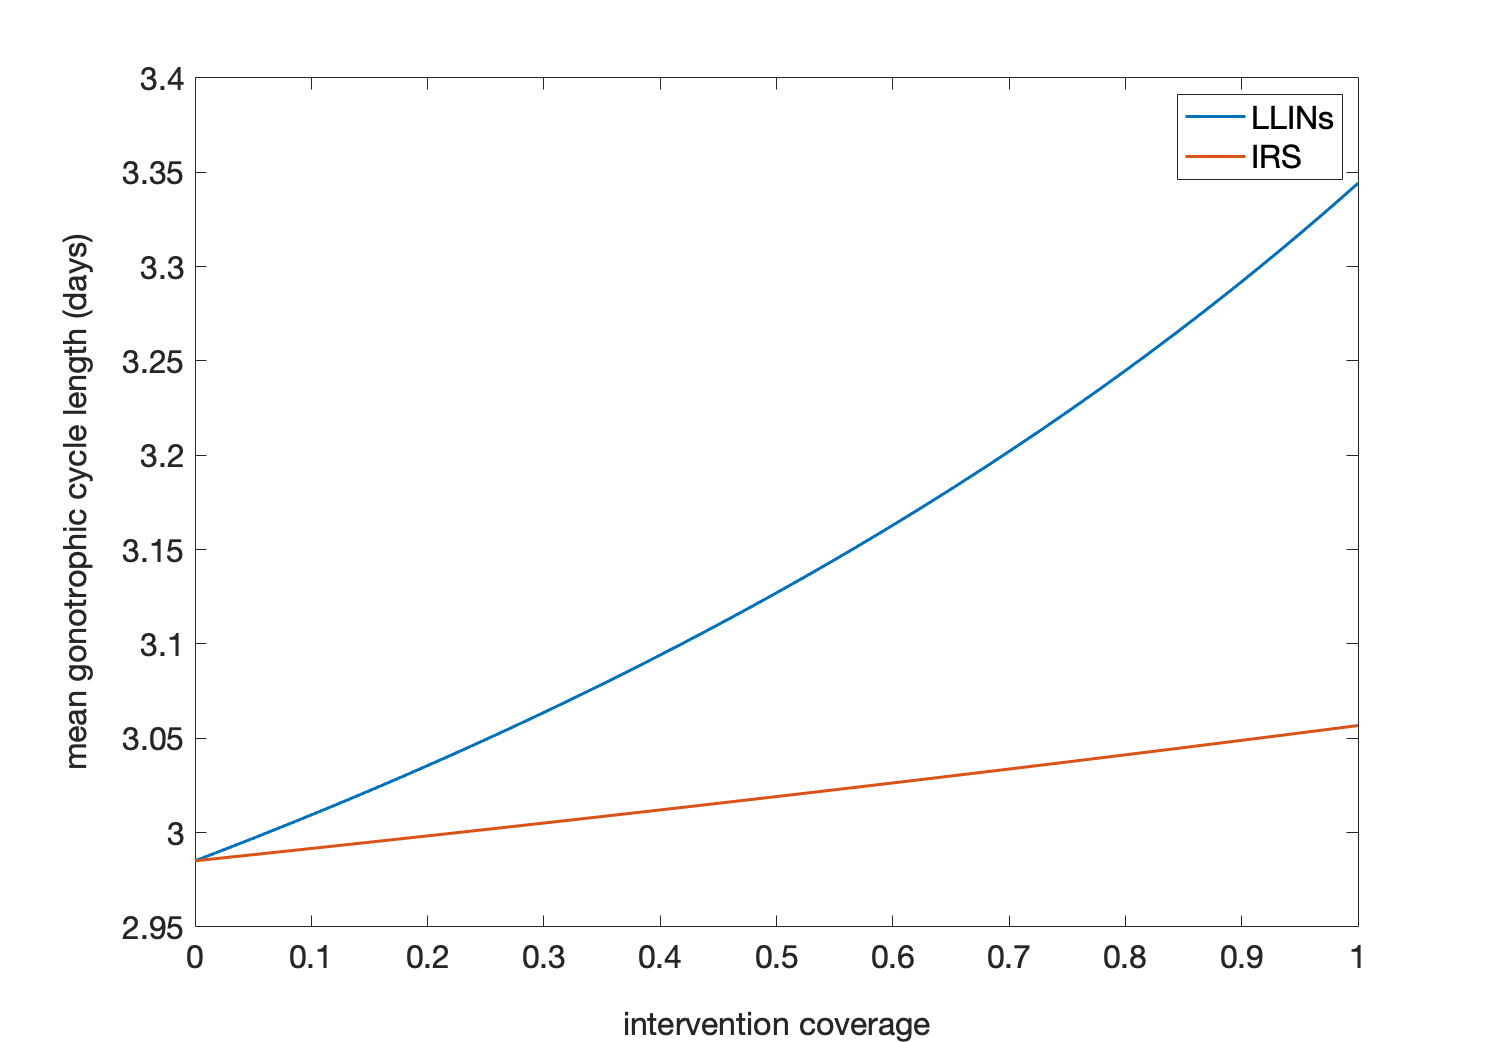
\includegraphics[height=6.7cm]{Project/Figures/VectorModel/LF/CycleLengthDays.png} & 
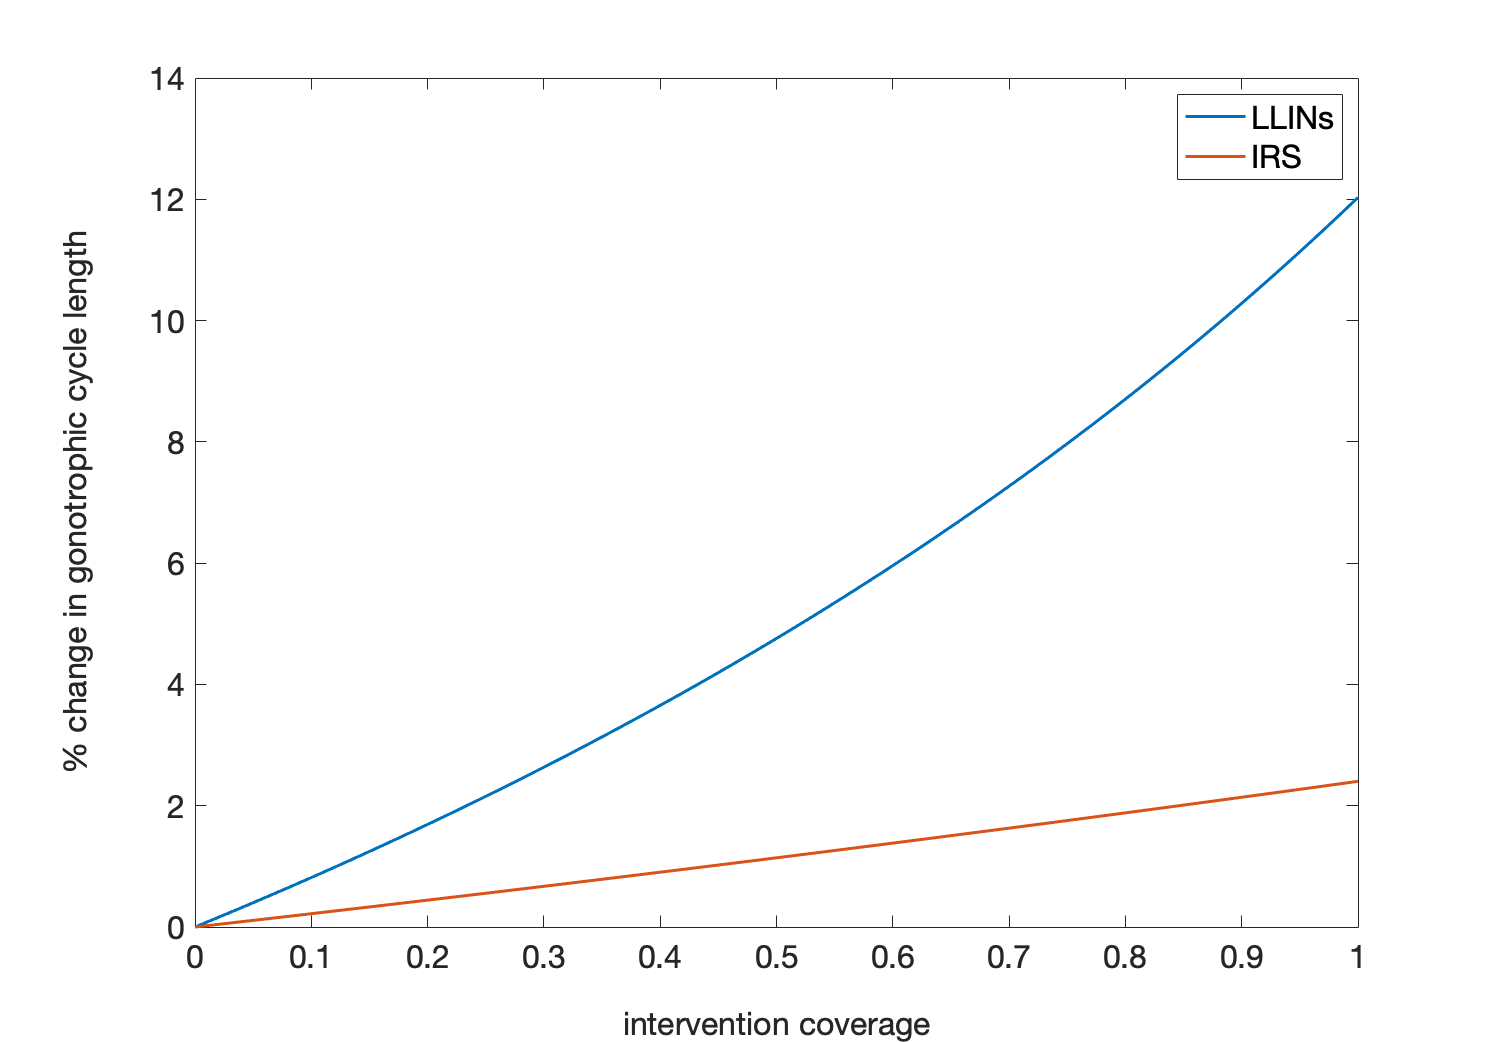
\includegraphics[height=6.7cm]{Project/Figures/VectorModel/LF/CycleLengthChange.png} \\
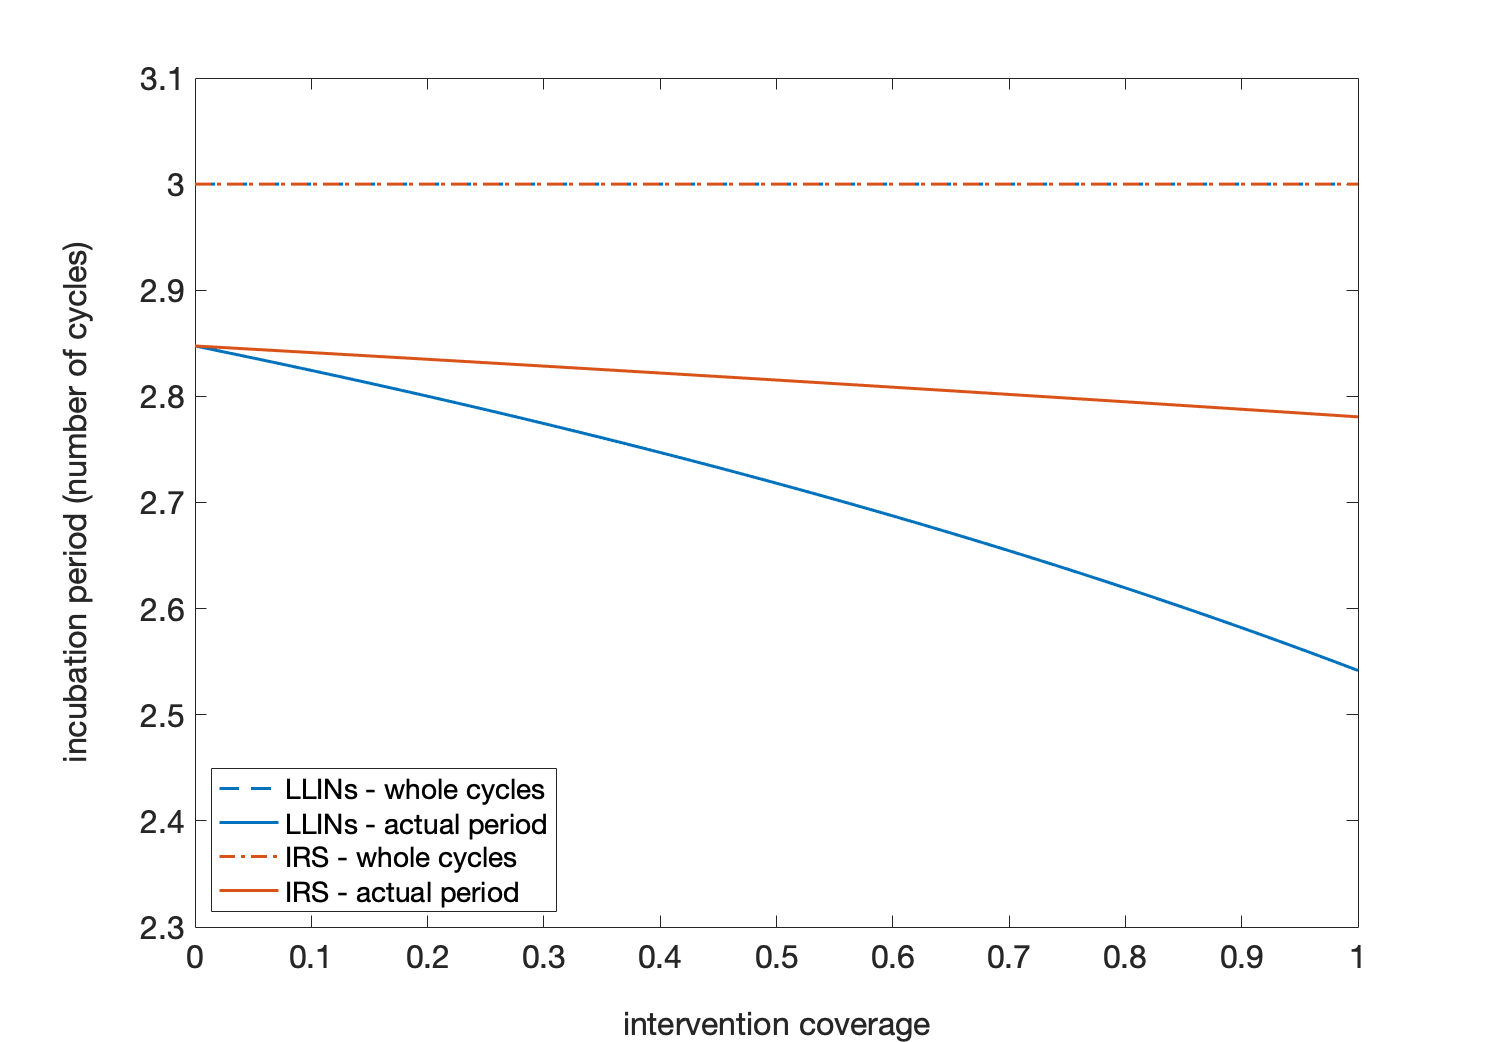
\includegraphics[height=6.7cm]{Project/Figures/VectorModel/LF/NumberCycles.png} &
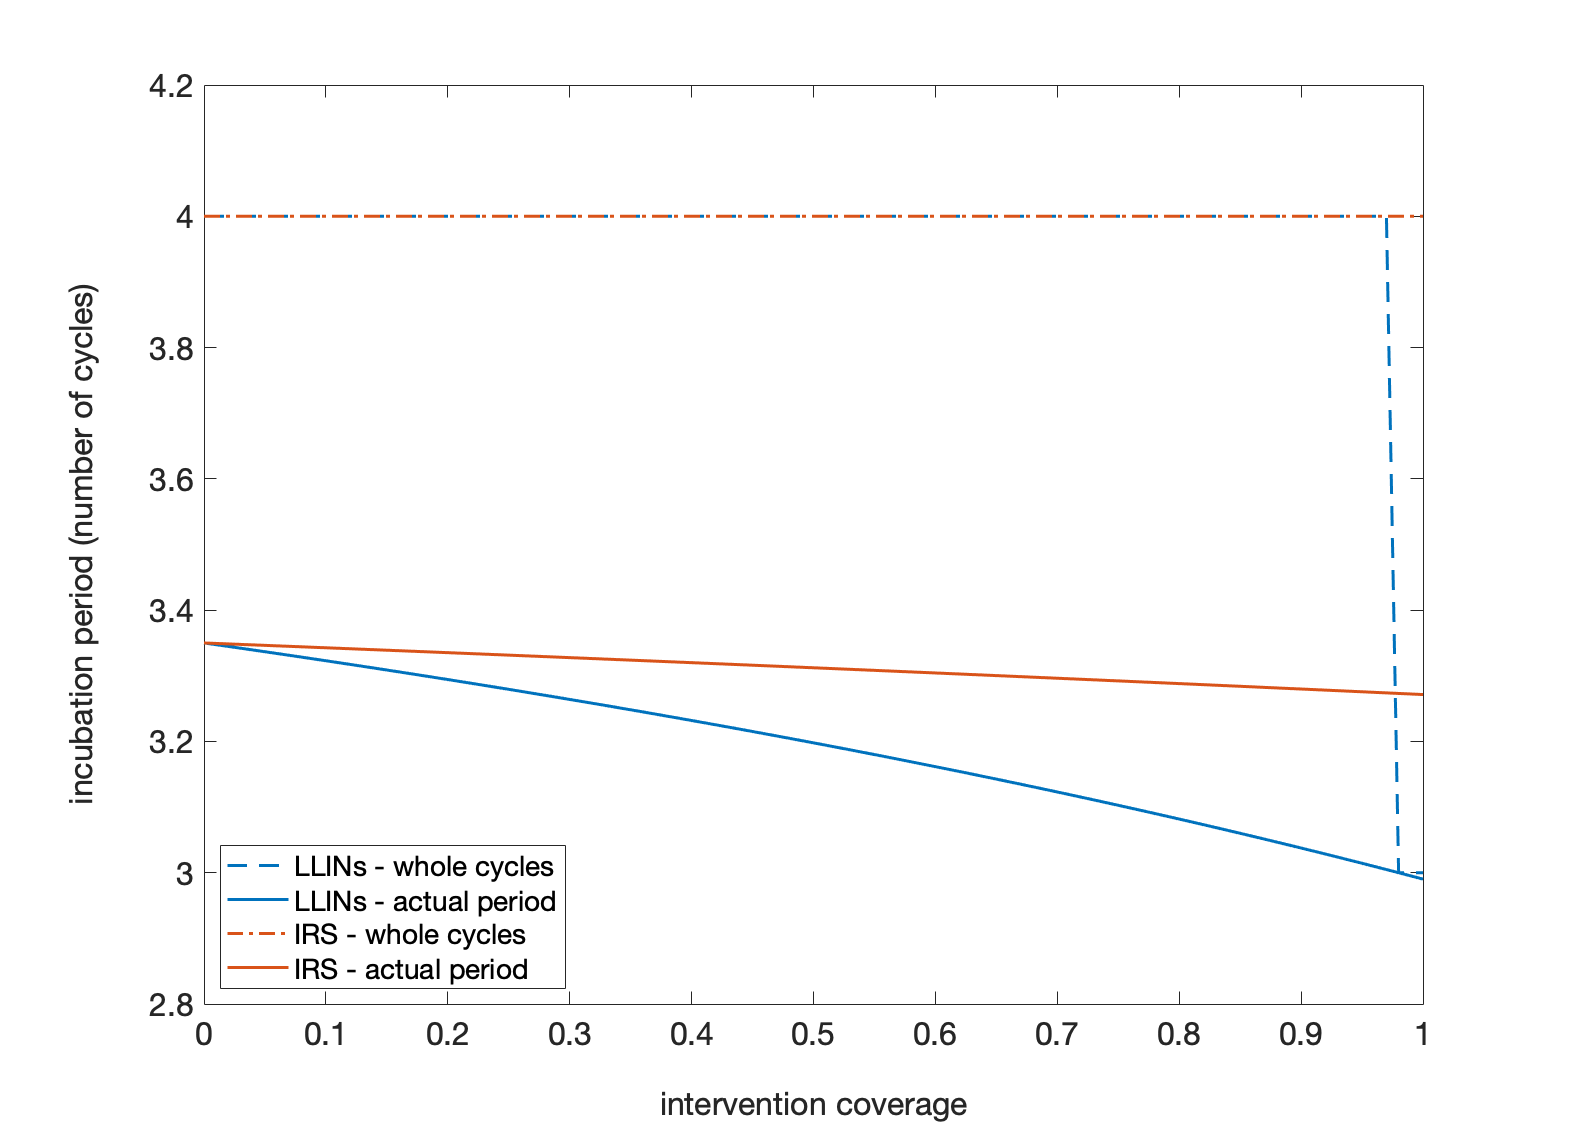
\includegraphics[height=6.7cm]{Project/Figures/VectorModel/Malaria/NumberCycles.png}
\end{array}$
\caption[Impact of repeating on gonotrophic cycle length.]{Cycle length plots for vector control interventions with repeating effects: LLINs (blue) and IRS (red). Top left: Mean change to gonotrophic cycle length (days). Top right: Percentage change in gonotrophic cycle length (\%). Both plots on the top row are independent of disease. Bottom left: Impact on incubation period in terms of the number of fractional (solid) and complete (dashed) cycles before infectiousness for lymphatic filariasis. Bottom right: Impact on incubation period in terms of the number of fractional (solid) and complete (dashed) cycles before infectiousness for malaria.}
\label{fig:cycles}
\end{center}
\end{sidewaysfigure} 

Figure \ref{fig:cycles} reiterates what we already saw in Figure \ref{fig:8controls_LF}, that LLINs have a much stronger repeating rate and this causes a larger increase in the gonotrophic cycle length. IRS can only cause at maximum just over a 2\% increase in mean cycle length, but high coverage of LLINs could lead to up to a 12\% increase. For LF (Figure \ref{fig:cycles} bottom left) the mean number of cycles required to pass through the EIP is around 2.85 in the presence of no interventions. A 12\% increase in cycle length results in an EIP which is still more than 2.5 cycles, hence three cycles are still required before a vector will be able to perform an infectious bite. Even 100\% coverage of LLINs is not sufficient to decrease the number of cycles required to reach infectivity.

For malaria (bottom right) LLINs are capable of bringing the EIP down from four cycles to three cycles, but only at very high coverage levels (greater than 95\%). As achieving 95\% LLIN coverage in practice is an unrealistic goal, this means that for the purposes of our results, the repeating effect has no change on the effective length of the incubation period in terms of generations of feeding, hence it is reasonable to take this parameter as fixed in the model for the purposes of our results. 

\subsection{Elimination settings}

As in Chapter \ref{chap:ELIM}, we are interested in elimination settings for LF, where we are either close to, or have achieved, a human prevalence of less than 1\% mf. Here we consider a setting where this reduction in prevalence has been caused largely by mass drug administration (MDA), rather than vector control measures. The impact of this on the vector dynamics can be simulated by considering a setting with the same vector to host ratio (or the same adult vector emergence rate) but a lower host prevalence. We are then interested in how using vector control measures will impact onward transmission.

\begin{sidewaysfigure}[p]
\begin{center}$
\begin{array}{cc}
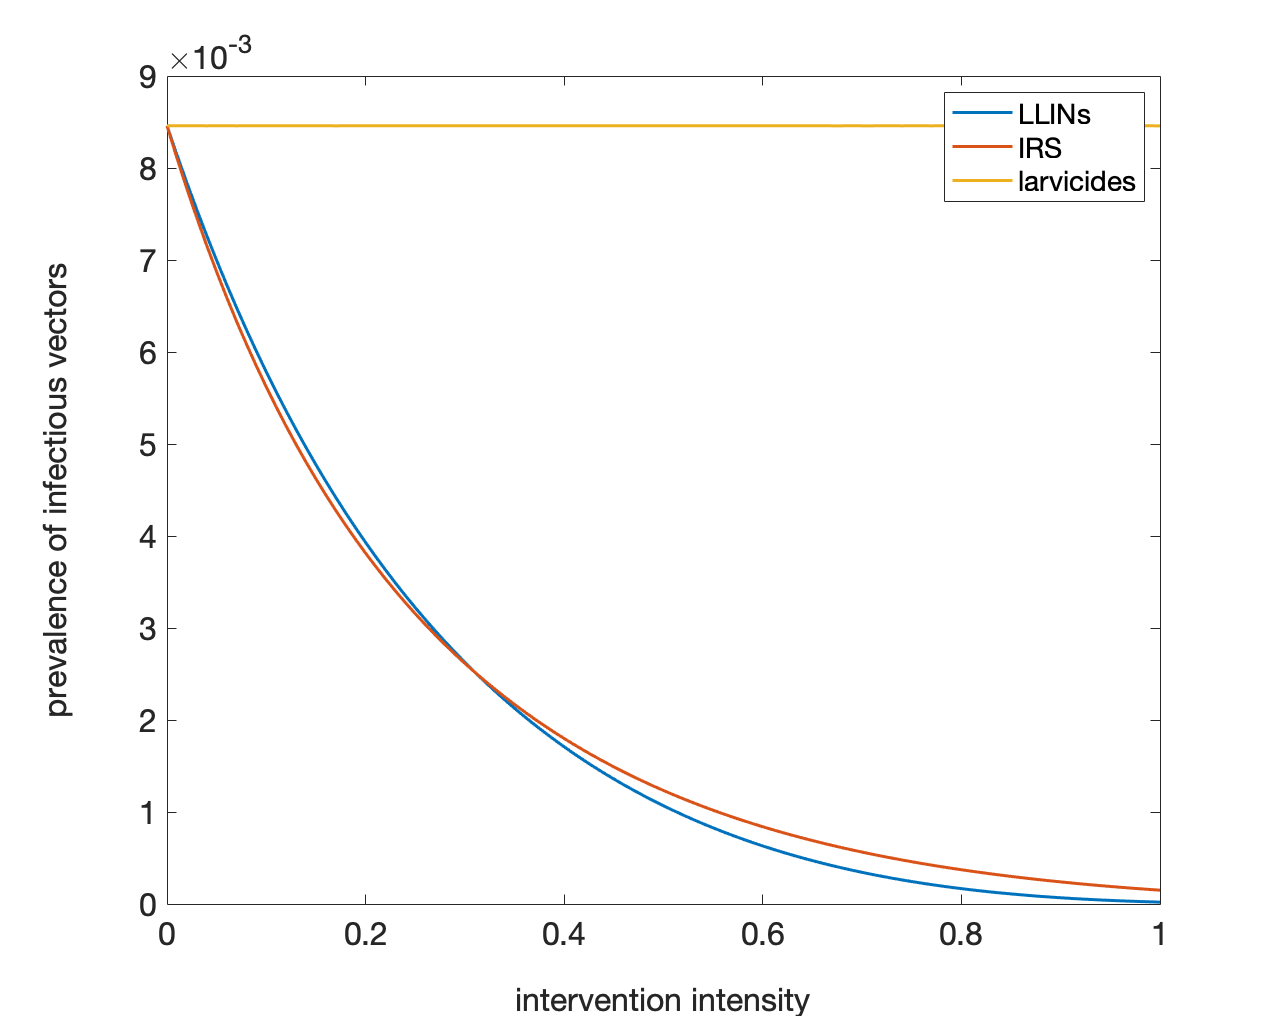
\includegraphics[height=8.5cm]{Project/Figures/VectorModel/LF/VecPrev_1mf.png} &
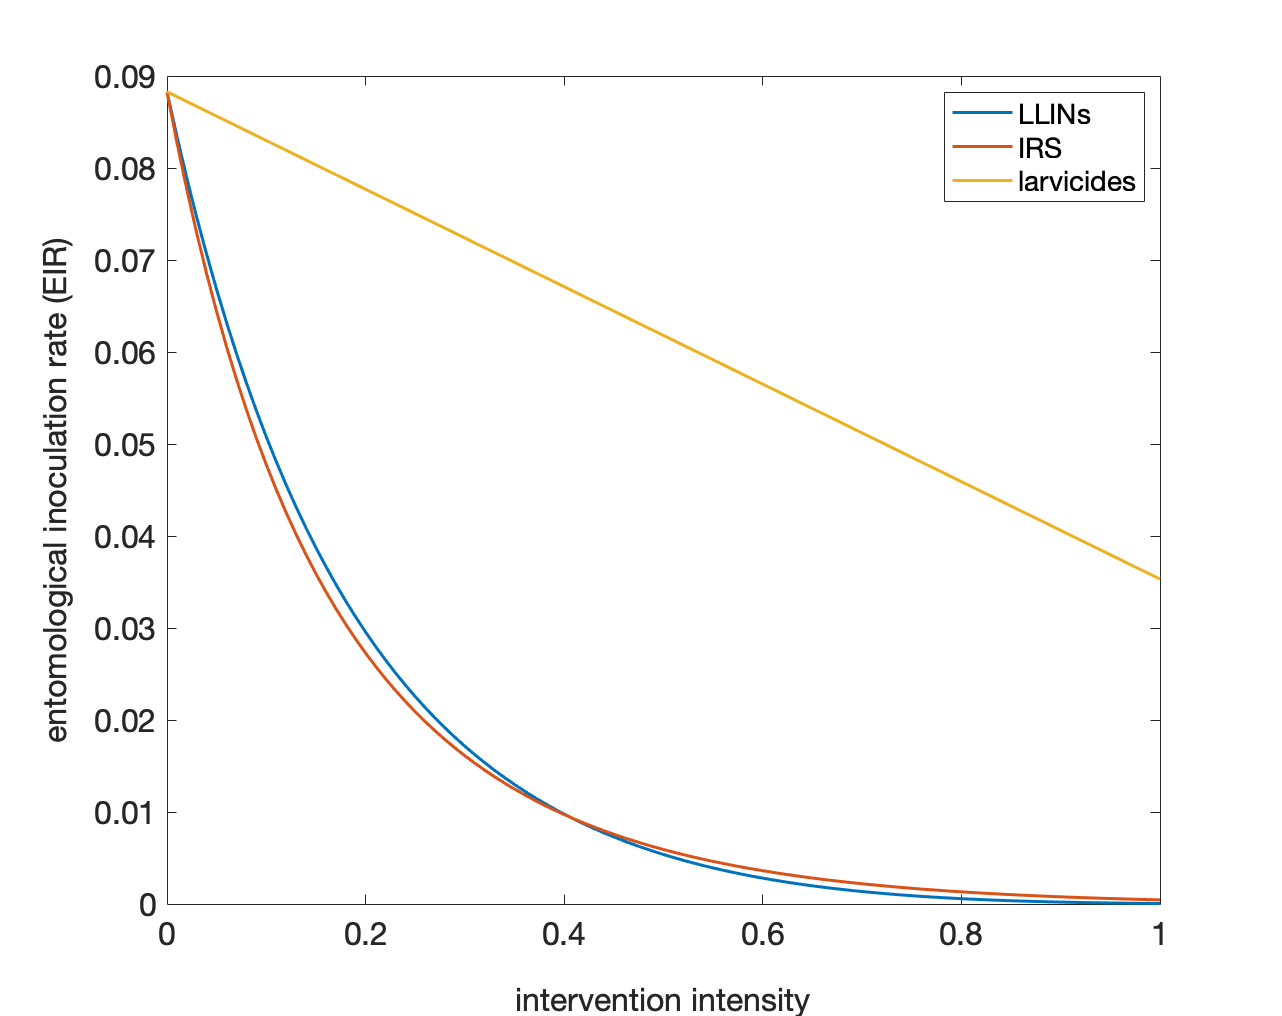
\includegraphics[height=8.5cm]{Project/Figures/VectorModel/LF/EIR_1mf.png}
\end{array}$
\caption[LF transmission measures at EPHP prevalence levels.]{Repeats of vector control intervention plots for the prevalence of infectiousness in vectors (left) and EIR (right) for LF with a host mf prevalence of 1\%. Other measures, including $R_e$, number of vectors in the population and vectorial capacity, are unchanged by the reduction in host prevalence.}
\label{fig:Elim_LF}
\end{center}
\end{sidewaysfigure} 

Transmission measures such as the basic reproductive number are independent of host prevalence, as they are defined based on one average infectious individual. However, the prevalence of infectious vectors and associated measures such as the EIR are substantially reduced by a reduction from 40\% to 1\% host prevalence (Figure \ref{fig:Elim_LF}).

When low host prevalences have been achieved it is highly important to maintain, and if possible improve on, these gains. In particular, adult-acting vector control measures and the impact they can have on $R_e$ could be vital in the final phases of elimination programs. 

\subsection{The Gambia}

Following on from the evidence of elimination discovered in The Gambia in the absence of MDA, I used the host infection process described in Section \ref{sec:Host} to investigate whether the model could achieve a prevalence of less than 1\% mf using just LLINs. I considered an equilibrium host mf prevalence of 50\%, which is reflective of measured mf levels in The Gambia in the 1950s, and then calculated the trend in human infection across ten years of consistent LLIN usage.

Figure \ref{fig:WM} shows the mean worm burden (W) and microfilaria count per 20$\mu$l of blood (M) decreasing over a ten year period in the presence of 40\% (left) and 80\% (right) LLIN coverage. There is a noticeable difference between the two levels of intervention and the decreasing mf levels appear to be reaching a plateau by the 10 year mark in both instances.

\begin{figure}[!ht]
\begin{center}$
\begin{array}{cc}
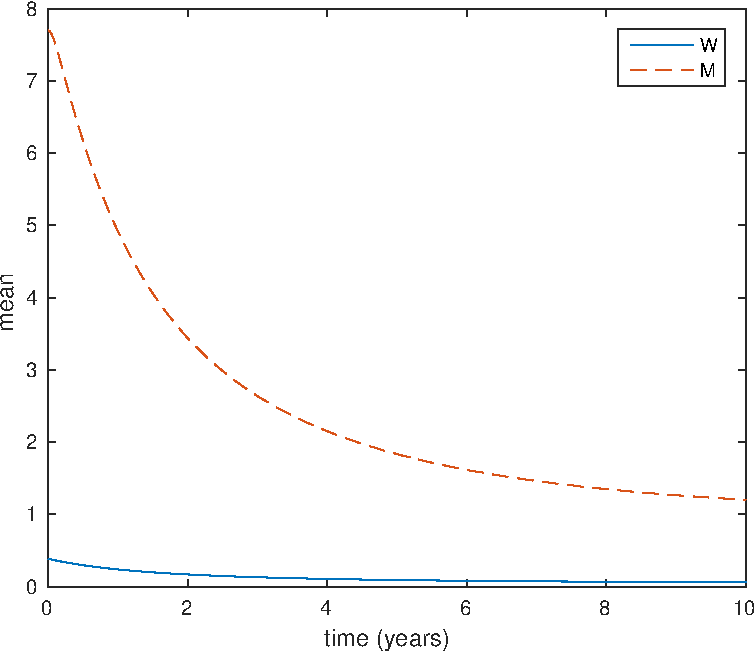
\includegraphics[height=5.8cm]{Project/Figures/VectorModel/LF/WM_1950s_omega=40per.pdf} &
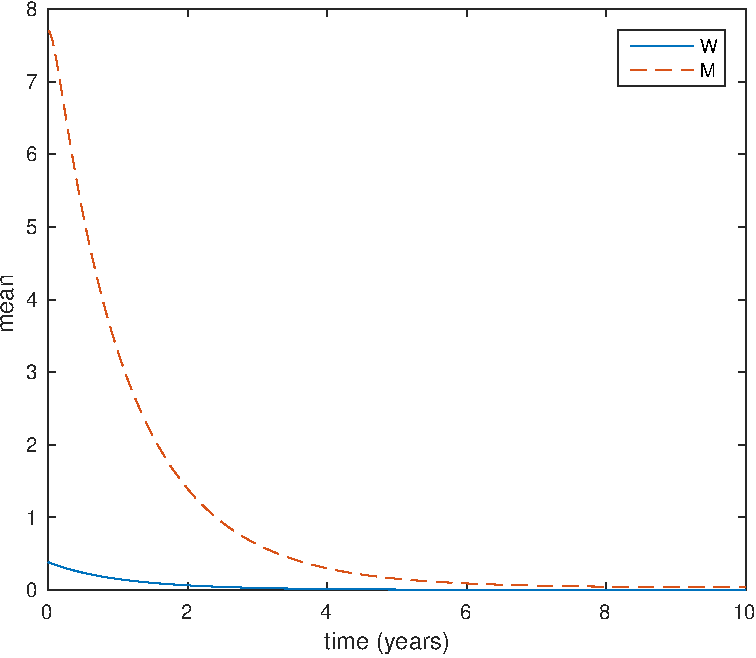
\includegraphics[height=5.8cm]{Project/Figures/VectorModel/LF/WM_1950s_omega=80per.pdf}
\end{array}$
\caption[LLIN impact over time (LF).]{Mean adult worm burden (W, blue solid) and mf count per 20$\mu$l of blood (M, red dashed) over ten years of LLIN usage at 40\% coverage (left) and 80\% coverage (right). Considering an equilibrium mf prevalence of 50\%, to reflect 1950s prevalence in The Gambia.}
\label{fig:WM}
\end{center}
\end{figure} 

Due to these apparent diminishing returns, we now consider the net benefit of 10 years of LLIN usage for a range of coverage, still given a starting mf prevalence of 50\% (Figure \ref{fig:10yrLLIN}). Looking at both the host and vector prevalences, we see the most substantial gains can be made by increasing coverage up to around 60\%; beyond this point increases in LLIN coverage have a much smaller relative effect. However, a coverage of 80\% or higher would be required to get host mf prevalence to below 1\% in this time period.

\begin{figure}[!ht]
\begin{center}
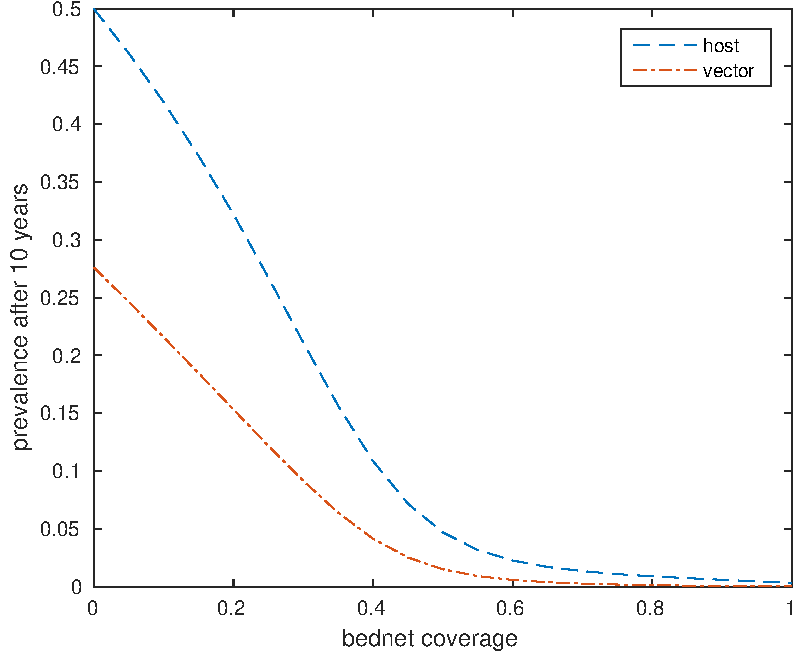
\includegraphics[height=8.5cm]{Project/Figures/VectorModel/LF/10yearprev_1950s_bednets.pdf} 
\caption[LLIN impact over 10 years (LF).]{Prevalence of LF in the host (blue dashed) and vector (red dot-dashed) after 10 years of LLIN usage for coverage between 0 and 100\%, starting at 50\% baseline mf prevalence.}
\label{fig:10yrLLIN}
\end{center}
\end{figure} 

\FloatBarrier

\section{Discussion}

The results presented in this chapter have used the explicit equilibrium solution of a gonotrophic cycle model for mosquito dynamics. Primarily the aim was to investigate how different vector control measures could change mosquito population structure and hence the potential effect on transmission of vector-borne diseases such as LF and malaria. We were also interested in the role long-lasting insecticidal nets may have played in the reduction of LF prevalence to below EPHP levels in The Gambia. We found that adult-acting vector control measures are likely to have a much greater effect on transmission than larval-based interventions. In particular, LLIN and IRS both have a compounded effect due to the repelling action reducing transmission both from host to vector and from vector to host. Areas that are co-endemic for malaria and LF, or other mosquito-borne diseases such as dengue, could especially benefit from adult-acting vector control. 

Considering the longitudinal usage of LLINs, the majority of reductions in mean worm burden and mf prevalence are achieved within 5 years of implementation. Even for relatively low LLIN coverage (40\%) a plateau begins to emerge around 10 years after implementation. Whilst we show that substantial reductions in mf prevalence could be caused by LLIN usage, we find that coverage may have to be unrealistically high (greater than 80\% of individuals sleeping under nets) to reproduce the results seen in The Gambia in the absence of other factors. This implies that LLINs may have played an important role in reducing prevalence across this over 50 year period, but that other environmental and social factors are also likely to have contributed to reducing transmission.

We assumed a number of things in the construction of this model, including a fixed EIP in the mosquito, that there is no impact of infection of vector fitness and that vector mortality remains constant with age. This last assumption is consistent with current understanding of wild mosquito populations; although senescence is observed in laboratory mosquitoes, wild mosquitoes are expected to die long before they can exhibit any substantial deterioration with age \cite{Ryan2015}. We also assumed that vector control interventions were maintained at the same coverage level across time, with no waning effects, which would be logistically difficult and expensive to achieve.

It is also important to remember that scale-ups in use of insecticides to combat transmission can result in wide-spread insecticide resistance and behavioral changes in sleeping conditions can lead to changes in biting behavior \cite{Fornadel2010,Weill2003}. These factors have the potential to undermine progress made using vector control measures, and in particular evidence of this has been seen in a number of malaria control programs \cite{Ranson2016,Hemingway2016,Toe2014}.

This model has been developed based on vector models in the malaria literature and hence makes no consideration of the parasite density dependent infectivity we expect to see for LF. In medium to high prevalence settings we would expect the probability of a mosquito becoming infected during an infectious blood meal to increase if the host has a higher worm burden. Future work could expand on the current model by considering the infection probability from host to vector as dependent on the mean filarial load, but would need more detailed data to parameterise this relationship. However, even with these limitations, considering the vector dynamics still provides important insight into how vector control measures could be explicitly described in established LF models.

Our results cover a range of high and medium transmission settings, briefly touching on a low prevalence setting of 1\%, but we do not consider host prevalences of less than 1\% mf. In the absence of explicit inclusion of the mating requirements for filarial worms, we would not expect to see the breakpoint described in Chapter \ref{chap:ELIM}. As this break point is often estimated as being below 1\% mf prevalence, we wouldn't expect this exclusion to have substantial impact on our presented results, although it is likely that vector control could prove a vital tool in the final stages of elimination.

As more countries begin to bring disease levels down towards the 1\% mf prevalence range, and target passing TAS, the key questions of importance change. Here we have presented a first investigation into how a range of vector control interventions could contribute towards the control and decline of disease prevalence in both the host and vector populations. The obvious follow-on question would be whether combining MDA and vector control could prove a useful tool. It would also be useful to investigate how progress can be maintained and furthered, and what role vector control should play in the next step of the journey towards elimination as we move away from intervention and more towards surveillance.

Post-MDA surveillance is a challenge facing a growing number of countries as more are validated for achieving EPHP. When prevalence is low there may be less adherence to vector control measures, but the vector is still an important marker of disease. A number of studies have suggested using xeno-monitoring as a method for detecting presence of disease in a population, but with a good enough understanding of disease it may be possible to link mf prevalence in humans to prevalence of infectious disease in mosquitoes \cite{Opoku2018,Pilotte2016}.

\subsection{Chapter summary}

In this chapter I gave an introduction to the literature on modelling malaria and LF. I then described the development of a deterministic compartmental model of the mosquito gonotrophic cycle, based on vector models used in the malaria literature. I incorporated vector control measures and infection dynamics into the model and investigated the impact of vector control on transmission. Adult-acting vector control was found be more effective than larvicide-based intervention for the same coverage level, due to the combination of adulticide and repelling effects. I also conclude that it is possible, but unlikely, that LLIN usage alone could be credited for a reduction to below EPHP levels of LF in The Gambia between 1950 and the present day.

%%
%% End of file `ejemplo latex RIAI.tex'.